%%%%%%%%%%%%%%%%%%%%%%%%%%%%%%%%%%%%%%%%%
% Masters/Doctoral Thesis 
% LaTeX Template
% Version 2.5 (27/8/17)
% Modified by udo mueller (2.3.2025)
%
% This template was downloaded from:
% http://www.LaTeXTemplates.com
%
% Version 2.x major modifications by:
% Vel (vel@latextemplates.com)
%
% This template is based on a template by:
% Steve Gunn (http://users.ecs.soton.ac.uk/srg/softwaretools/document/templates/)
% Sunil Patel (http://www.sunilpatel.co.uk/thesis-template/)
%
% Template license:
% CC BY-NC-SA 3.0 (http://creativecommons.org/licenses/by-nc-sa/3.0/)
%
%%%%%%%%%%%%%%%%%%%%%%%%%%%%%%%%%%%%%%%%%

%----------------------------------------------------------------------------------------
%	PACKAGES AND OTHER DOCUMENT CONFIGURATIONS
%----------------------------------------------------------------------------------------

\documentclass[
11pt, % The default document font size, options: 10pt, 11pt, 12pt
%oneside, % Two side (alternating margins) for binding by default, uncomment to switch to one side
english, % ngerman for German
singlespacing, % Single line spacing, alternatives: onehalfspacing or doublespacing
%draft, % Uncomment to enable draft mode (no pictures, no links, overfull hboxes indicated)
%nolistspacing, % If the document is onehalfspacing or doublespacing, uncomment this to set spacing in lists to single
%liststotoc, % Uncomment to add the list of figures/tables/etc to the table of contents
%toctotoc, % Uncomment to add the main table of contents to the table of contents
%parskip, % Uncomment to add space between paragraphs
%nohyperref, % Uncomment to not load the hyperref package
headsepline, % Uncomment to get a line under the header
%chapterinoneline, % Uncomment to place the chapter title next to the number on one line
%consistentlayout, % Uncomment to change the layout of the declaration, abstract and acknowledgements pages to match the default layout
]{MastersDoctoralThesis} % The class file specifying the document structure

\usepackage[utf8]{inputenc} % Required for inputting international characters
\usepackage[T1]{fontenc} % Output font encoding for international characters

\usepackage{mathpazo} % Use the Palatino font by default

% use listings package for programming languages
\usepackage{listings}

% Package for landscape orientation
\usepackage{pdflscape}

% Setup glossaries
\usepackage[automake,acronym]{glossaries}
\makeglossaries
\loadglsentries{glossary}

% Use the bober backend with the authoryear citation style 
% (which resembles APA)
% Use the biber backend instead of bibtex whenever possible.
% This adds unicode support
\usepackage[backend=biber, style=ieee, natbib=true, citestyle=numeric-comp]{biblatex}
% TODO use IEEE ok?
% \usepackage[backend=biber,style=authoryear,natbib=true]{biblatex} 

\addbibresource{thesis.bib} % The filename of the bibliography

\usepackage[autostyle=true]{csquotes} % Required to generate language-dependent quotes in the bibliography

%----------------------------------------------------------------------------------------
%	MARGIN SETTINGS
%----------------------------------------------------------------------------------------

\geometry{
	paper=a4paper, % Change to letterpaper for US letter
	inner=2.5cm, % Inner margin
	outer=3.8cm, % Outer margin
	bindingoffset=.5cm, % Binding offset
	top=1.5cm, % Top margin
	bottom=1.5cm, % Bottom margin
	%showframe, % Uncomment to show how the type block is set on the page
}

%----------------------------------------------------------------------------------------
%	THESIS INFORMATION
%----------------------------------------------------------------------------------------

\thesistitle{Generative AI for Security Automation in Hyperscale Cloud Platforms} % Your thesis title, this is used in the title and abstract, print it elsewhere with \ttitle

\supervisor{Prof. Udo \textsc{Müller}} % Your supervisor's name, this is used in the title page, print it elsewhere with \supname

\examiner{} % Your examiner's name, this is not currently used anywhere in the template, print it elsewhere with \examname

\degree{Master of Business Information Systems} % Your degree name, this is used in the title page and abstract, print it elsewhere with \degreename

\author{Daniel \textsc{Vera Gilliard}} % Your name, this is used in the title page and abstract, print it elsewhere with \authorname

\addresses{} % Your address, this is not currently used anywhere in the template, print it elsewhere with \addressname

\subject{Business Information Systems} % Your subject area, this is not currently used anywhere in the template, print it elsewhere with \subjectname

\keywords{} % Keywords for your thesis, this is not currently used anywhere in the template, print it elsewhere with \keywordnames

\university{\href{http://www.h-ka.de}{Hochschule Karlsruhe}} % Your university's name and URL, this is used in the title page and abstract, print it elsewhere with \univname
\department{\href{http://department.university.com}{Business Information Systems}} % Your department's name and URL, this is used in the title page and abstract, print it elsewhere with \deptname

\group{\href{http://researchgroup.university.com}{Research Group Name}} % Your research group's name and URL, this is used in the title page, print it elsewhere with \groupname

\faculty{\href{http://faculty.university.com}{Faculty Name}} % Your faculty's name and URL, this is used in the title page and abstract, print it elsewhere with \facname

\AtBeginDocument{
\hypersetup{pdftitle=\ttitle} % Set the PDF's title to your title
\hypersetup{pdfauthor=\authorname} % Set the PDF's author to your name
\hypersetup{pdfkeywords=\keywordnames} % Set the PDF's keywords to your keywords
}



\usepackage{tikz}

\usepackage{tgheros}
\renewcommand*\familydefault{\sfdefault}



\begin{document}

\include{Frontpage/Frontpage}

%----------------------------------------------------------------------------------------
%	DECLARATION PAGE
%----------------------------------------------------------------------------------------

\begin{declaration}
\addchaptertocentry{\authorshipname} % Add the declaration to the table of contents

\noindent I, \authorname,
in lieu of an oath that I have written the Master's thesis presented
here independently and exclusively using the literature and other aids
provided. The thesis has not been submitted in the same or a similar form
to any other examination authority for the award of an academic degree.

 \vskip20pt

\noindent Signed:\\
\rule[0.5em]{25em}{0.5pt} % This prints a line for the signature
 
 \vskip10pt
\noindent Date:\\
\rule[0.5em]{25em}{0.5pt} % This prints a line to write the date
\end{declaration}

\cleardoublepage


% This goes in the body of your .tex document where you want the declaration to appear.
\begin{customdeclaration}{Declaration on the Use of Generative AI}
\addcontentsline{toc}{chapter}{Declaration on the Use of Generative AI}

\noindent I, \authorname, hereby declare that generative artificial intelligence (AI) was employed as a writing assistant in the development of this manuscript. The use of these tools was exclusively for linguistic enhancement, such as refining sentence structure, correcting grammar, and improving overall style. The conceptual framework, original ideas, research methodology, data analysis, and final conclusions presented in this work are the product of my own intellectual effort. I have critically reviewed, edited, and validated all content to ensure its accuracy and originality, and I bear complete responsibility for the entirety of this thesis.

\vspace{2cm}

\noindent\makebox[2.5cm]{Signed:} \rule[0.5em]{12cm}{0.5pt}

\vspace{1.5cm}

\noindent\makebox[2.5cm]{Date:} \rule[0.5em]{12cm}{0.5pt}

\end{customdeclaration}

\cleardoublepage

%----------------------------------------------------------------------------------------
%	QUOTATION PAGE
%----------------------------------------------------------------------------------------

\vspace*{0.2\textheight}

\noindent\enquote{\itshape Thanks to my solid academic training, today I can write hundreds of words on virtually any topic without possessing a shred of information, which is how I got a good job in journalism.}\bigbreak

\hfill Dave Barry



%----------------------------------------------------------------------------------------
%	ABSTRACT PAGE
%----------------------------------------------------------------------------------------

\begin{abstract}
\addchaptertocentry{\abstractname} % Add the abstract to the table of contents
This thesis addresses the challenge of automating cloud security policy generation using Generative AI (GenAI), focusing on the integration of Large Language Models (LLMs) with traditional static analysis in a Retrieval-Augmented Generation (RAG) framework. Motivated by the need for scalable, context-aware, and reliable security automation in complex cloud environments, the research follows a Design Science Research paradigm, progressing through literature review, conceptual framework development, prototype implementation, and empirical evaluation.

The primary contributions are: (1) a novel conceptual framework that combines the speed of static analysis with the contextual reasoning of LLMs, grounded in curated data and validated through a Human-in-the-Loop (HITL) process; and (2) a functional prototype empirically evaluated on Infrastructure-as-Code for AWS using Terraform and tfsec. Results demonstrate measurable improvements in policy efficacy, generation speed, and contextual detection quality compared to static-only baselines, while highlighting the necessity of human oversight for nuanced decision-making.

The findings advance the shift-left security paradigm by providing a blueprint for embedding automated, preventative controls early in the development lifecycle. Limitations include the narrow technology focus and prototype scope, suggesting future research directions in broader stack generalization and GenAI optimization. This work offers a practical guide for integrating GenAI into DevSecOps pipelines, bridging the gap between rapid development and robust security assurance.
\end{abstract}



%----------------------------------------------------------------------------------------
%	ACKNOWLEDGEMENTS
% Not required in Germany; write if you feel it appropriate
%----------------------------------------------------------------------------------------

\begin{acknowledgements}
\addchaptertocentry{\acknowledgementname} % Add the acknowledgements to the table of contents
The acknowledgments and the people to thank go here, don't forget to include your project advisor\ldots
\end{acknowledgements}




%----------------------------------------------------------------------------------------
%	LIST OF CONTENTS/FIGURES/TABLES PAGES
%----------------------------------------------------------------------------------------

\tableofcontents % Prints the main table of contents

\listoffigures % Prints the list of figures

\listoftables % Prints the list of tables

%----------------------------------------------------------------------------------------
%	Listings of programs - neccessary if you have any program texts
%----------------------------------------------------------------------------------------
\lstlistoflistings

%----------------------------------------------------------------------------------------
%	ABBREVIATIONS - not neccessary if you do not have any not well known abbreviations
%----------------------------------------------------------------------------------------

\begin{abbreviations}{ll} % Include a list of abbreviations (a table of two columns)

\textbf{ABAC} & \textbf{A}ttribute-\textbf{B}ased \textbf{A}ccess \textbf{C}ontrol\\
\textbf{ACSC} & \textbf{A}ustralian \textbf{C}yber \textbf{S}ecurity \textbf{C}entre\\
\textbf{AI} & \textbf{A}rtificial \textbf{I}ntelligence\\
\textbf{AI RMF} & \textbf{A}rtificial \textbf{I}ntelligence \textbf{R}isk \textbf{M}anagement \textbf{F}ramework\\
\textbf{APP} & \textbf{A}ustralian \textbf{P}rivacy \textbf{P}rinciples\\
\textbf{CIA} & \textbf{C}onfidentiality, \textbf{I}ntegrity, and \textbf{A}vailability\\
\textbf{CSP} & \textbf{C}loud \textbf{S}ervice \textbf{P}rovider\\
\textbf{DTA} & \textbf{D}igital \textbf{T}ransformation \textbf{A}gency\\
\textbf{GenAI} & \textbf{Gen}erative \textbf{A}rtificial \textbf{I}ntelligence\\
\textbf{LLM} & \textbf{L}arge \textbf{L}anguage \textbf{M}odel\\
\textbf{MLOps} & \textbf{M}achine \textbf{L}earning \textbf{Op}erations\\
\textbf{MTTD} & \textbf{M}ean \textbf{T}ime \textbf{t}o \textbf{D}etect\\
\textbf{MTTR} & \textbf{M}ean \textbf{T}ime \textbf{t}o \textbf{R}esolve\\
\textbf{RAG} & \textbf{R}etrieval-\textbf{A}ugmented \textbf{G}eneration\\
\textbf{RPO} & \textbf{R}ecovery \textbf{P}oint \textbf{O}bjectives\\
\textbf{RTO} & \textbf{R}ecovery \textbf{T}ime \textbf{O}bjectives\\
\textbf{SOC} & \textbf{S}ecurity \textbf{O}perations \textbf{C}enter\\
\textbf{SRM} & \textbf{S}hared \textbf{R}esponsibility \textbf{M}odel\\
\textbf{WAF} & \textbf{W}eb \textbf{A}pplication \textbf{F}irewalls\\
\textbf{ZTA} & \textbf{Z}ero \textbf{T}rust \textbf{A}rchitecture\\

\end{abbreviations}

%----------------------------------------------------------------------------------------
%	PHYSICAL CONSTANTS/OTHER DEFINITIONS - not neccessary if you do not have any
%----------------------------------------------------------------------------------------

\begin{constants}{lr@{${}={}$}l} % The list of physical constants is a three column table

% The \SI{}{} command is provided by the siunitx package, see its documentation for instructions on how to use it

Speed of Light & $c_{0}$ & \SI{2.99792458e8}{\meter\per\second} (exact)\\
%Constant Name & $Symbol$ & $Constant Value$ with units\\

\end{constants}

%----------------------------------------------------------------------------------------
%	SYMBOLS - not neccessary if you do not have any
%----------------------------------------------------------------------------------------

\begin{symbols}{lll} % Include a list of Symbols (a three column table)

$a$ & distance & \si{\meter} \\
$P$ & power & \si{\watt} (\si{\joule\per\second}) \\
%Symbol & Name & Unit \\

\addlinespace % Gap to separate the Roman symbols from the Greek

$\omega$ & angular frequency & \si{\radian} \\

\end{symbols}



% Print the glossaries
\printglossaries

%----------------------------------------------------------------------------------------
%	DEDICATION
%----------------------------------------------------------------------------------------

\dedicatory{For/Dedicated to/To my\ldots} 




%----------------------------------------------------------------------------------------
%	THESIS CONTENT - CHAPTERS
%----------------------------------------------------------------------------------------

\mainmatter % Begin numeric (1,2,3...) page numbering

\pagestyle{thesis} % Return the page headers back to the "thesis" style

% Include the chapters of the thesis as separate files from the Chapters folder
% Uncomment the lines as you write the chapters

% Chapter 1

\chapter{Introduction}
\label{chap:introduction}

%----------------------------------------------------------------------------------------

% Define some commands to keep the formatting separated from the content 
\newcommand{\keyword}[1]{\textbf{#1}}
\newcommand{\tabhead}[1]{\textbf{#1}}
\newcommand{\code}[1]{\texttt{#1}}
\newcommand{\file}[1]{\texttt{\bfseries#1}}
\newcommand{\option}[1]{\texttt{\itshape#1}}

%----------------------------------------------------------------------------------------

% Section 1.1: Start with the broad context and then narrow down to the specific problem.
% Context: The increasing adoption of hyperscale cloud platforms and Infrastructure-as-Code (IaC).
% Problem: The scale and complexity of these environments make manual security analysis and policy creation slow, error-prone, and insufficient for modern DevSecOps cycles.
\section{Motivation and Problem Statement}
\label{sec:motivation_problem}
% In this section, introduce the convergence of GenAI and cloud security.
% State the core problem: the need for advanced automation to analyze IaC configurations and proactively generate preventative security controls to keep pace with rapid development cycles.

TBD

% Section 1.2: Clearly state what this thesis aims to achieve and the questions it seeks to answer.
% This should be derived from your work in Chapters 4 and 5.
\section{Research Objectives and Questions}
\label{sec:objectives_questions}

This thesis explores how Generative AI (GenAI) can help solve the security challenges in modern cloud environments. The research focuses on using GenAI to automate security tasks and asks the following central question:

\textit{How can Generative AI technologies be effectively leveraged to automate security operations across hyperscale cloud platforms?}

To comprehensively answer this overarching question, the research is decomposed into three distinct but interrelated areas, each addressed by a set of specific sub-questions.

The first area of investigation focuses on establishing a foundational understanding of the current landscape. This involves a systematic analysis of the state of the art to examine the existing research and implementation of GenAI for security automation at hyperscale cloud providers. This analysis compares existing GenAI toolsets and models across major cloud platforms and identifies the primary limitations and challenges in current GenAI implementations for cloud security. This foundational work is primarily addressed in the literature review presented in Chapter \ref{chap:Background and Related Work}.

The second area of investigation concerns the design of an innovative solution. The goal is to develop a conceptual framework that operationalizes GenAI for security automation. This requires exploring how GenAI can be specifically applied to automate policy generation and management, what architecture is required for effective multi-cloud policy orchestration using GenAI, and what validation mechanisms are necessary to ensure trust and accuracy in GenAI-driven security automation. These questions guide the development of the conceptual framework detailed in Chapter \ref{chap:conceptual_framework}.

Finally, the third area addresses the practical implementation and empirical validation of the proposed framework. This involves determining which technical approach is most effective for implementing GenAI-driven security automation across hyperscale cloud platforms and how the effectiveness of such a system can be measured and validated. Furthermore, this research seeks to understand what balance between automation and human oversight optimizes security outcomes in a real-world context. These questions are addressed through the prototype implementation described in Chapter \ref{chap:implementation} and the evaluation of its results, which will be presented in Chapter \ref{chap:results}.

By methodically addressing these questions, this thesis aims to provide a comprehensive, empirically grounded contribution to the field of automated cloud security.

% Section 1.3: Explain the unique contribution of your work.
% Your main contributions are the conceptual framework (Ch 4) and the prototype implementation (Ch 5).
\section{Contribution and Significance}
\label{sec:contribution}
% Detail the key contributions:
% 1. A novel conceptual framework for GenAI-driven security automation that integrates static analysis, a RAG-based LLM approach, and a multi-stage validation process.
% 2. The design and implementation of a prototype system that validates this framework using industry-standard technologies (AWS, Terraform, OPA).
% Explain the significance: This work advances "shift-left" security, provides a practical blueprint for integrating GenAI into DevSecOps pipelines, and reduces the manual burden on security teams.

TBD

% Section 1.4: Briefly explain HOW you will answer your research questions.
% This should be a high-level summary of the approach detailed in Chapter 3 and executed in Chapters 4-6.
\section{Methodology Overview}
\label{sec:methodology_overview}
% Briefly describe your research approach. For example, mention that the thesis follows a design science methodology, involving:
% 1. A comprehensive literature review to identify research gaps (Chapter 2).
% 2. The development of a conceptual framework (Chapter 4).
% 3. The implementation of a functional prototype (Chapter 5).
% 4. An evaluation of the prototype against defined metrics such as policy efficacy and generation speed (Chapter 6).

TBD or separate section?

% Section 1.5: Give the reader a roadmap of the entire thesis.
% This is a summary of each chapter's purpose.
\section{Outline of the Thesis}
\label{sec:outline}
% Briefly describe the content and purpose of each subsequent chapter.
% For example:
% \textbf{Chapter 2} provides a comprehensive background on foundational concepts in cloud security and GenAI, reviews the state of the art in related work, and identifies the research gaps that this thesis addresses.
% \textbf{Chapter 3} outlines the research methodology employed in this work.
% \textbf{Chapter 4} introduces the conceptual framework for GenAI-driven security automation, detailing its multi-layered architecture, the integration of LLMs, and the Human-in-the-Loop workflow.
% \textbf{Chapter 5} describes the practical implementation of the framework as a prototype, covering the system architecture, technology stack, and end-to-end workflow.
% \textbf{Chapter 6} presents the results from the evaluation of the prototype based on the metrics defined in the framework.
% \textbf{Chapter 7} discusses the implications of the results, connecting them back to the research questions and the existing literature.
% \textbf{Chapter 8} concludes the thesis by summarizing the key findings, acknowledging limitations, and suggesting directions for future research.

TBD
% Chapter 2

\chapter{Background and Related Work} % (fold)
\label{chap:Background and Related Work}

\section{Foundational Concepts in Cloud Computing} % (fold)
\label{sec:Foundational Concepts in Cloud Computing}

TBD

% section Foundational Concepts in Cloud Computing (end)

\section{Foundational Concepts in Generative AI} % (fold)
\label{sec:Foundational Concepts in Generative AI}

TBD

% section Foundational Concepts in Generative AI (end)

\section{State of Cloud Provider Ecosystems} % (fold)
\label{sec:State of Cloud Provider Ecosystems}

TBD

% section State of Cloud Provider Ecosystems (end)

\section{Literature State of the Art} % (fold)
\label{sec:State of the Art}

The convergence of Generative Artificial Intelligence (GenAI) and hyperscale cloud platforms presents a rapidly evolving frontier for cybersecurity. As organizations increasingly rely on complex cloud environments, the scale and sophistication of threats necessitate advanced automation capabilities. GenAI offers promising avenues for enhancing security posture through intelligent automation, but its integration also introduces challenges and risks. A comprehensive understanding of the existing research landscape is therefore essential to identify established practices, emerging trends, and critical gaps in knowledge.

This literature review synthesizes current academic and industry contributions pertinent to the application of GenAI for security automation within hyperscale and multi-cloud contexts. It begins by outlining the methodology employed to select and analyze relevant works. Subsequently, the review dives into several key thematic areas: the evolution from traditional security methods to AI-driven approaches, specific frameworks for scoping and managing GenAI security implementations, architectural patterns and techniques for security automation, a critical examination of the unique security risks associated with GenAI itself, risk management frameworks and the ongoing crucial discussion regarding the necessary balance between automation and human oversight.

By examining these facets, this review aims to provide a foundational understanding of the state-of-the-art, highlighting both the potential of GenAI in cloud security automation and the significant considerations that must be addressed for its responsible and effective deployment. This synthesis will inform the subsequent research presented in this thesis.
% Soll das Kapitel ein State of the Art sein, oder auch ein Review. Weil wenn es ein Review ist, dann %könntest du manche Paper noch etwas kritischer hinterfragen. Stärken Schwächen. 

\subsection{Methodology} % (fold)
\label{sec:Methodology}

This literature review followed a structured approach to identify relevant publications, focusing on peer-reviewed articles addressing GenAI applications in hyperscale cloud security published primarily within the last five years. The search utilized academic databases with key search terms related to generative AI, cloud security automation, hyperscale platforms, and multi-cloud orchestration.
Papers were selected based on their relevance to:

\begin{itemize}
\item GenAI applications specifically in cloud security contexts
\item Hyperscale or multi-cloud environments
\item Technical solutions for security automation
\item Empirical evidence or theoretical frameworks with substantial methodological rigor
\end{itemize}

The selection process involved initial screening of titles and abstracts followed by full-text review of promising papers. The analysis employed a thematic approach, identifying recurring concepts, methodological approaches, and gaps in existing research. Particular attention was paid to identifying the theoretical foundations underpinning GenAI applications in security contexts, empirical evidence of effectiveness, and limitations of current approaches.

% subsection Methodology (end)

\subsection{AI-Driven Security Approaches} % (fold)
\label{sec:AI-Driven Security Approaches}

The landscape of cloud security is undergoing a significant transformation, shifting from traditional, often reactive methods towards more proactive and adaptive strategies powered by Artificial Intelligence (AI), particularly Generative AI (GenAI). This evolution marks a move beyond basic anomaly detection towards sophisticated security postures capable of learning from and responding dynamically to novel threat vectors in complex cloud environments.

Foundational work by Khanna \cite{khanna_enhancing_2024} explores the integration of GenAI into cloud security, outlining its core applications. According to Khanna, modern GenAI implementations focus on key capabilities such as processing vast amounts of data (e.g., log entries, network packets) for advanced anomaly detection and threat intelligence, enabling automated response mechanisms that dynamically adjust security protocols, and facilitating predictive security measures to forecast potential vulnerabilities. While highlighting these advancements, Khanna also acknowledges inherent challenges, including the need for large datasets and mitigating potential adversarial manipulation \cite{khanna_enhancing_2024}.

Building upon these foundational capabilities, the integration of GenAI represents a significant leap beyond conventional rule-based security systems. Research indicates that GenAI enhances security automation, particularly within multi-cloud and hybrid architectures. It allows systems to adapt infrastructure dynamically in response to varying traffic patterns and implements AI-powered defenses against continuously evolving cyber threats. This adaptive capability directly addresses persistent challenges in cloud security related to optimizing workload distribution, ensuring performance, and managing costs effectively \cite{seth_ai_2025}.

Furthermore, recent studies underscore the practical impact of integrating GenAI with established cloud-native security tools. Patel et al. \cite{patel_generative_2025} demonstrate how layering GenAI onto platforms like AWS GuardDuty and Google Cloud Security Command Center significantly boosts automated threat detection, enables real-time incident response, and improves comprehensive vulnerability management across distributed cloud infrastructures. Their work provides empirical evidence, citing examples like Netflix and JPMorgan Chase, which reported measurable improvements in detection accuracy and notable reductions in security incidents following the adoption of GenAI-driven security automation strategies \cite{patel_generative_2025}. This convergence of GenAI with existing security frameworks highlights its potential to transform security operations centers (SOCs) by enhancing both efficiency and effectiveness.

% subsection AI-Driven Security Approaches (end)

\subsection{GenAI Security Frameworks}
\label{sec:GenAI Security Frameworks}

Addressing the unique security challenges posed by Generative AI (GenAI) requires structured approaches and comprehensive frameworks. These help organizations assess risks, implement controls, and ensure compliance throughout the AI lifecycle.
One foundational approach is the "Generative AI Security Scoping Matrix," provided by AWS, which offers a structured framework for assessing security requirements based on the \textit{type} of GenAI deployment\cite{noauthor_securing_nodate}. This framework aids organizations in evaluating their security posture, identifying potential vulnerabilities, and implementing appropriate controls throughout the AI lifecycle\cite{noauthor_securing_nodate}. While core security disciplines remain essential, the matrix specifically helps address the unique risks and additional considerations introduced by generative AI workloads\cite{noauthor_securing_nodate}. It classifies implementations into five scopes, representing increasing levels of ownership and control\cite{noauthor_securing_2023}:

\begin{enumerate}
    \item \textbf{Consumer apps (Scope 1):} Utilising public third-party GenAI services (e.g., public chatbots), often with no cost or paid access, where the business does not own or see the training data or model and cannot modify it. Interaction occurs via APIs or direct application use according to provider terms\cite{noauthor_securing_2023}\cite{noauthor_securing_nodate}. This falls under the "Buying" category of GenAI usage\cite{noauthor_securing_nodate}.
    \item \textbf{Enterprise apps (Scope 2):} Employing third-party enterprise applications (e.g., Amazon Q) with embedded GenAI features, involving an established business relationship with the vendor\cite{noauthor_securing_2023}\cite{noauthor_securing_nodate}. This also falls under the "Buying" category\cite{noauthor_securing_nodate}.
    \item \textbf{Pre-trained models (Scope 3):} Building custom applications that integrate with existing third-party foundation models (e.g., Amazon Bedrock base models) via APIs\cite{noauthor_securing_2023}\cite{noauthor_securing_nodate}. This represents the start of the "Building" category\cite{noauthor_securing_nodate}.
    \item \textbf{Fine-tuned models (Scope 4):} Refining an existing third-party foundation model by fine-tuning it with business-specific data, resulting in a new, specialized model (e.g., Amazon Bedrock customized models)\cite{noauthor_securing_2023}\cite{noauthor_securing_nodate}. This is part of the "Building" category\cite{noauthor_securing_nodate}.
    \item \textbf{Self-trained models (Scope 5):} Constructing and training a GenAI model from the ground up using proprietary or acquired data, implying full ownership of the model (e.g., using Amazon SageMaker)\cite{noauthor_securing_2023}\cite{noauthor_securing_nodate}. This represents the highest level of ownership in the "Building" category\cite{noauthor_securing_nodate}.
\end{enumerate}
This matrix serves as a mental model\cite{noauthor_securing_nodate} that helps security teams prioritize focus areas by identifying five key security disciplines whose requirements vary across the deployment scopes: governance and compliance, legal and privacy, risk management, controls, and resilience\cite{noauthor_securing_2023}\cite{noauthor_securing_nodate}. As organizations move across the scopes from consuming consumer apps (Scope 1) towards building self-trained models (Scope 5), the demands within these disciplines evolve significantly. For instance, governance requirements escalate from basic compliance with terms of service to comprehensive frameworks for model development and monitoring. Similarly, risk management priorities shift, potentially focusing on prompt injection for pre-trained models (Scope 3) versus data poisoning or model extraction for fine-tuned or self-trained models (Scopes 4 and 5). The necessary security controls also transition from emphasizing access policies in lower scopes to implementing technical safeguards like adversarial testing and output filtering in higher scopes. Resilience planning also adapts based on the application's criticality. By mapping their GenAI activities to this matrix, organizations can systematically assess risks and apply appropriate security measures tailored to their specific implementation context.

Building upon such scoping considerations, more comprehensive frameworks aim to provide detailed security blueprints. A notable contribution to the field is the SecGenAI framework, which provides a comprehensive approach to securing cloud-based Generative AI (GenAI) applications, with particular attention to Retrieval-Augmented Generation (RAG) systems within the context of Australian Critical Technologies of National Interest\cite{haryanto_secgenai_2024}. This framework addresses the unique security challenges introduced by the rapid advancement of GenAI technologies\cite{haryanto_secgenai_2024}.
SecGenAI is structured around three core pillars: functional, infrastructure, and governance requirements\cite{haryanto_secgenai_2024}. It integrates an end-to-end security analysis to generate detailed specifications. These specifications emphasize critical areas such as data privacy, secure deployment methodologies, and the implementation of shared responsibility models between cloud service providers and users\cite{haryanto_secgenai_2024}. The framework's development addresses key questions surrounding GenAI security, the requirements for Confidentiality, Integrity, and Availability, specific RAG implementation options, constraints within the Australian regulatory landscape, and alignment with ethical principles\cite{haryanto_secgenai_2024}.
A key aspect of SecGenAI is its alignment with established Australian guidelines, including the Australian Privacy Principles (APP) \cite{resources_australias_2024}, particularly APP 11 concerning the security of personal information, Australia's AI Ethics Principles \cite{resources_australias_2024}, and guidance from the Australian Cyber Security Centre (ACSC) and the Digital Transformation Agency\cite{haryanto_secgenai_2024}. This alignment ensures that security measures incorporate regulatory compliance without hindering operational efficiency\cite{haryanto_secgenai_2024}. The framework specifically targets GenAI-specific threats that often evade traditional security countermeasures. These threats include data leakage (potentially revealing sensitive training or knowledge base data), various adversarial attacks (such as prompt injection, data poisoning, and model inversion techniques designed to extract underlying data or manipulate outputs), jailbreaking attacks (bypassing content restrictions), and the potential for GenAI to generate insecure code or be misused by threat actors\cite{haryanto_secgenai_2024}. SecGenAI proposes a multi-layered security strategy combining advanced machine learning techniques with robust security measures.

Functional Security Requirements:
\begin{itemize}
    \item \textbf{Identity and Access Management:} Utilizing continuous and adaptive authentication mechanisms, alongside Attribute-Based Access Control (ABAC), to manage user access dynamically based on behavior and context\cite{haryanto_secgenai_2024}.
    \item \textbf{Data Confidentiality and Integrity:} Employing techniques like homomorphic encryption to process encrypted data, data masking and tokenization to protect sensitive information, and data integrity verification using methods like hashing and artificial fingerprinting\cite{haryanto_secgenai_2024}.
    \item \textbf{Model Security:} Implementing adversarial attack mitigation, encrypting model parameters, and ensuring secure model training protocols, potentially using differential privacy or federated learning\cite{haryanto_secgenai_2024}.
\end{itemize}

Infrastructure Security Requirements:
\begin{itemize}
    \item Implementing sandboxed environments often within dedicated cloud availability zones and virtual private networks\cite{haryanto_secgenai_2024}.
    \item Securing database connections using read replicas, strict IAM policies, and robust encryption methods\cite{haryanto_secgenai_2024}.
    \item Establishing stringent network security settings, segregating internal and external connections, and utilizing security groups\cite{haryanto_secgenai_2024}.
    \item Deploying external attack prevention mechanisms like Web Application Firewalls (WAF) and DDoS mitigation services, potentially integrated with data processing and monitoring tools (e.g., AWS Kinesis, Glue, Athena, Grafana)\cite{haryanto_secgenai_2024}.
    \item Ensuring robust data backup and disaster recovery strategies, considering Recovery Time Objectives (RTO) and Recovery Point Objectives (RPO)\cite{haryanto_secgenai_2024}.
\end{itemize}

Governance Requirements:
\begin{itemize}
    \item Adhering to AI governance principles (based on the ISO 38500 Evaluate-Direct-Monitor cycle \cite{noauthor_isoiec_nodate}) covering fairness, accountability, content traceability (e.g., watermarking), data protection, regular audits, reliability, user consent, third-party risk management, transparency, and legal compliance\cite{haryanto_secgenai_2024}.
    \item Clearly defining roles and responsibilities through an AI-specific Shared Responsibility Model (SRM) for cloud environments, outlining obligations for Cloud Service Providers (CSPs), customers, and areas of shared duty\cite{haryanto_secgenai_2024}.
\end{itemize}
By addressing these functional, infrastructure, and governance aspects in detail, the SecGenAI framework provides actionable strategies for the secure implementation and operation of cloud-based GenAI systems, fostering innovation while safeguarding national interests and enhancing the overall reliability and trustworthiness of these transformative technologies\cite{haryanto_secgenai_2024}.

Furthermore, as organizations increasingly adopt multi-cloud strategies, effective policy orchestration across diverse environments becomes critical for maintaining consistent security postures and operational efficiency\cite{sushil_prabhu_prabhakaran_integration_2024}. A comprehensive analysis of unified AI and cloud platforms published in 2024 examines architectural frameworks and integration patterns that enable the convergence of AI tools, machine learning operations (MLOps), data processing systems, and workflow orchestration within cloud-native environments, primarily focusing on transforming process automation and decision systems\cite{sushil_prabhu_prabhakaran_integration_2024}. This research investigates how these unified platforms address challenges like managing distributed AI workloads, ensuring real-time processing, and maintaining regulatory compliance\cite{sushil_prabhu_prabhakaran_integration_2024}.
This research identifies three key innovations within these unified platforms with significant implications for advanced automation, including security automation:
\begin{itemize}
    \item \textbf{Federated AI implementations:} These allow organizations to train AI models across distributed nodes or cloud boundaries while preserving data sovereignty and privacy, as sensitive data does not need to be centralized. This approach also reduces network bandwidth requirements and utilizes techniques like secure aggregation protocols and differential privacy\cite{sushil_prabhu_prabhakaran_integration_2024}.
    \item \textbf{Real-time data processing architectures:} Leveraging advanced streaming technologies (like Apache Kafka or Flink), in-memory processing, and real-time analytics engines, these architectures enable sub-second decision-making and immediate response to events (such as potential threats) by efficiently handling continuous data streams with high reliability and fault tolerance\cite{sushil_prabhu_prabhakaran_integration_2024}.
    \item \textbf{Multi-cloud integration patterns:} These patterns establish standardized interfaces, communication protocols, service discovery mechanisms, load balancing, and security controls to ensure seamless and consistent operation, including policy enforcement, across different cloud providers. Hybrid cloud deployment strategies are also highlighted, intelligently distributing workloads between on-premise and cloud resources based on performance, cost, and compliance needs, managed by sophisticated orchestration\cite{sushil_prabhu_prabhakaran_integration_2024}.
\end{itemize}
These architectural approaches, integrating MLOps frameworks for lifecycle management, robust data processing, workflow orchestration, and advanced capabilities like federated learning and real-time analytics within a multi-cloud context, provide the necessary foundation upon which advanced solutions like GenAI-driven security automation can be built across heterogeneous cloud environments\cite{sushil_prabhu_prabhakaran_integration_2024}. While the analyzed paper focuses broadly on process automation and decision systems, the detailed exploration of scalable, resilient, governable, and interoperable architectures directly supports the implementation of sophisticated, automated security measures in complex multi-cloud settings\cite{sushil_prabhu_prabhakaran_integration_2024}.

% subsection GenAI Security Frameworks (end) 

\subsection{Approaches for Automated Cloud Security} % (fold)
\label{sec:Approaches for Automated Cloud Security}

This subsection details specific technical approaches and architectural patterns crucial for enabling automated cloud security. It reviews research on unified platforms integrating AI and MLOps across multi-cloud environments, techniques for automated policy orchestration in complex Kubernetes setups, and the application of digital twins for robust security policy validation. These approaches represent concrete mechanisms for realizing the potential of automation in dynamic cloud infrastructures.

For organizations operating containerized workloads across multiple clusters, particularly in multi-domain architectures involving different administrative entities, research from 2023 proposes an automated approach for generating network security policies in Kubernetes deployments\cite{bringhenti_security_2023}. Manually configuring security in such environments is complex, often leading to inconsistencies between policies defined in different clusters and requiring domain administrators to possess knowledge about other domains' configurations (like service locations or IP addresses), which is not always feasible\cite{bringhenti_security_2023}. This approach addresses two critical challenges in multi-cluster security: reducing the configuration errors commonly made by human administrators and creating transparent cross-cluster communications without requiring extensive information sharing between domains\cite{bringhenti_security_2023}.

The proposed solution involves a top-level entity named the "Multi-Cluster Orchestrator"\cite{bringhenti_security_2023}. This orchestrator acts as a central management point, receiving inputs from managers of different domains\cite{bringhenti_security_2023}. These inputs include:
\begin{itemize}
    \item A description of each domain's structure (listing clusters and exposed services with their details)\cite{bringhenti_security_2023}.
    \item High-level security requirements specifying allowed communications (e.g., between services within the same domain, services in different domains, or services and external IP addresses)\cite{bringhenti_security_2023}. These requirements can be defined using an extended YAML syntax with special labels (`service`, `cluster`, `domain`) that abstract away low-level details\cite{bringhenti_security_2023}.
\end{itemize}

Based on these inputs, the Multi-Cluster Orchestrator refines the high-level requirements into concrete configurations through a two-step process\cite{bringhenti_security_2023}:
\begin{enumerate}
    \item It generates a "Global Configuration" that tracks communication pairs between services and required links between clusters, optimizing the overall cluster mesh setup\cite{bringhenti_security_2023}.
    \item It derives "Single Configurations" for each individual cluster, containing the specific parameters needed to connect the cluster to the mesh (e.g., using technologies like Cilium Cluster Mesh), the Kubernetes Network Policies to enforce the desired security rules, and commands to create local service entries that enable transparent name resolution for services located in external clusters\cite{bringhenti_security_2023}.
\end{enumerate}

The implementation, known as Multi-Cluster Orchestrator (developed in Java with REST APIs), demonstrates how automated policy generation can improve security consistency across distributed environments while reducing the cognitive load on security administrators by handling the complexity of multi-domain interactions transparently\cite{bringhenti_security_2023}. This research is particularly relevant for hyperscale cloud platforms and organizations that utilize container orchestration technologies like Kubernetes to manage numerous workloads across multiple clusters, potentially spanning different regions, availability zones, or administrative boundaries\cite{bringhenti_security_2023}.

Another approach to security automation in the context of policies involves the use of digital twins for validating security policies before deployment in production environments\cite{hammar_digital_2023}. This approach utilizes an emulation system specifically designed to create high-fidelity digital replicas of target IT infrastructures\cite{hammar_digital_2023}. These digital twins replicate key functionalities of the corresponding physical or virtual systems, allowing security teams to play out complex security scenarios, such as intrusion attempts and defense responses, within a safe and controlled environment\cite{hammar_digital_2023}. This capability avoids impacting operational workflows on the real-world infrastructure\cite{hammar_digital_2023}.

The digital twin approach, following the research by Hammar and Stadler, enables a closed-loop learning process for crafting and refining security policies\cite{hammar_digital_2023}. It starts with generating a digital twin of the target infrastructure. This is achieved using an emulation system constructed with virtualization tools like Docker containers, alongside virtual links and switches\cite{hammar_digital_2023}. Within this digital twin, various security scenarios involving emulated attackers, defenders, and client populations are executed\cite{hammar_digital_2023}. During these runs, monitoring agents collect detailed system measurements and logs, channeling this data through pipelines for analysis\cite{hammar_digital_2023}. The gathered data and statistics are then used to build simulations\cite{hammar_digital_2023}. Reinforcement learning techniques are applied to these simulations to learn potentially optimal security policies\cite{hammar_digital_2023}. Finally, the performance of these learned policies is rigorously evaluated back in the digital twin, allowing for validation and further iteration\cite{hammar_digital_2023}.

This methodology provides continuous, iterative feedback and improvement cycles, as the results from validation can inform further scenario runs and learning phases, enhancing policy effectiveness over time\cite{hammar_digital_2023}. The authors demonstrate this by applying the approach to an intrusion response scenario, showing that the digital twin provided the necessary evaluative feedback to learn near-optimal policies that outperformed baseline systems like the SNORT IDPS\cite{zhou_study_2010}. This represents a significant advancement in validation mechanisms, particularly relevant for potentially complex GenAI-driven security automation strategies, by bridging the gap between simulation-based learning and real-world applicability\cite{hammar_digital_2023}.

Regarding policies, ensuring the trustworthiness and accuracy of GenAI-generated security policies and responses remains a significant challenge. The already mentioned SecGenAI framework demonstrates how advanced machine learning techniques can be combined with robust security measures to enhance the reliability of GenAI systems while maintaining compliance with regulatory requirements.\cite{haryanto_secgenai_2024}
As described, this approach integrates continuous validation processes throughout the AI lifecycle, from model development to deployment and monitoring, creating multiple checkpoints that verify the integrity and effectiveness of security responses. By emphasizing explainability alongside accuracy, the framework addresses one of the primary concerns associated with GenAI applications in security contexts: the "black box" nature of complex models.\cite{haryanto_secgenai_2024}

While not specifically focused on cloud security, research on GenAI applications in the energy sector offers transferable insights into implementation approaches for complex operating environments. This comprehensive literature review identifies how GenAI enhances productivity through data creation, forecasting, optimization, and natural language understanding, while also addressing challenges such as hallucinations, data biases, privacy concerns, and system errors \cite{surathunmanun_exploring_2024}.
The proposed solutions—including improving training data quality, implementing system fine-tuning processes, establishing human oversight mechanisms, and deploying robust security measures—provide a valuable framework for GenAI implementations in cloud security contexts. These approaches are particularly relevant for hyperscale environments where scale and complexity amplify both the benefits and risks of GenAI adoption \cite{surathunmanun_exploring_2024}.

% subsection Approaches for Automated Cloud Security (end)

\subsection{Agent-Based Approaches} % (fold)
\label{sec:Agent-Based Approaches}

A recent paper from 2024 introduces and validates the concept of employing Generative AI (GenAI)-driven agentic workflows to achieve comprehensive security automation, particularly in complex modern environments. A notable example is the DevSecOps Sentinel system\cite{noauthor_devsecops_nodate}, specifically designed to address the mounting security challenges inherent in modern software supply chains. Challenges coming from microservices, containerization, and cloud-native architectures that often outpace traditional DevSecOps practices\cite{noauthor_devsecops_nodate}.

The DevSecOps Sentinel system exemplifies this approach by utilizing intelligent agents integrated into automated workflows. These agents are powered by advanced GenAI models, such as Large Language Models (LLMs) enhanced with Retrieval-Augmented Generation (RAG), enabling sophisticated analysis capabilities\cite{noauthor_devsecops_nodate}. Key characteristics of these agents include:

\begin{itemize}
    \item \textbf{Autonomy:} Operating independently based on predefined goals and policies.
    \item \textbf{Reactivity:} Responding in real-time to environmental changes like new vulnerability disclosures.
    \item \textbf{Proactivity:} Taking initiative, such as preemptively scanning for risks or suggesting improvements\cite{noauthor_devsecops_nodate}.
\end{itemize}

These agents execute critical security tasks throughout the software development lifecycle, including:

\begin{itemize}
    \item \textbf{Automated Vulnerability and Impact Analysis:} Leveraging GenAI to analyze code, dependencies (tracked via SBOMs), and infrastructure configurations for potential threats, assessing their potential impact in context\cite{noauthor_devsecops_nodate}.
    \item \textbf{Adaptive Compliance and Release Gating:} Enforcing security policies and compliance requirements dynamically, acting as automated checks before deployment\cite{noauthor_devsecops_nodate}.
    \item \textbf{Predictive Security:} Utilizing AI to identify potential future risks based on historical data and emerging threat patterns\cite{noauthor_devsecops_nodate}.
\end{itemize}

The implementation and testing of DevSecOps Sentinel demonstrate several key points relevant to broader security automation:

\begin{enumerate}
    \item \textbf{Viability for Complexity:} Agentic workflows powered by GenAI are shown to be a viable and effective method for tackling the intricate and rapidly evolving security issues found in modern, distributed systems\cite{noauthor_devsecops_nodate}.
    \item \textbf{Synergy of AI and Agents:} The integration of GenAI's deep analysis capabilities with the autonomous, proactive nature of agentic systems offers a powerful paradigm for strengthening organizational security posture\cite{noauthor_devsecops_nodate}. While Sentinel focuses on the supply chain, the principle applies broadly to automating security operations in complex cloud environments.
    \item \textbf{Measurable Improvements:} Such systems can contribute to building and deploying software that is simultaneously faster, safer, and more reliable. The DevSecOps Sentinel study reported significant quantitative improvements in key security and operational metrics, including reduced Mean Time to Detect (MTTD) and Resolve (MTTR) for vulnerabilities, lower false positive rates, increased compliance pass rates, higher deployment frequency, and reduced change failure rates\cite{noauthor_devsecops_nodate}.
\end{enumerate}

This approach, exemplified by DevSecOps Sentinel, highlights a promising direction for leveraging GenAI to automate and enhance security functions, moving beyond traditional limitations to offer more adaptive, context-aware, and efficient security management in demanding environments like hyperscale clouds.

% subsection Agent-Based Approaches (end)

\subsection{Security Risks} % (fold)
\label{sec:Security Risks}

The increasing integration of Generative Artificial Intelligence (GenAI) into various domains, including cybersecurity, presents significant opportunities but also introduces complex and multifaceted risks. Insights from recent literature reviews highlight these emerging challenges. A systematic literature review by Nyoto et al. \cite{nyoto_cyber_2024}, analyzing 17 relevant studies according to PRISMA 2020 guidelines \cite{page_prisma_2021}, identifies several significant cybersecurity threats stemming primarily from the irresponsible application of GenAI technology. Complementing this, Surathunmanun et al. \cite{surathunmanun_exploring_2024}, while reviewing GenAI in the energy sector, outline key challenges that possess direct and critical relevance to security implementations, particularly within cloud environments reliant on third-party models and data. Synthesizing these findings provides a comprehensive overview of the risks:

\begin{itemize}
    \item \textbf{Enhanced Malicious Content Generation and Misuse:} GenAI significantly lowers the barrier for creating sophisticated malicious content and tools. It can be abused to generate highly personalized and convincing phishing messages and social engineering tactics, increasing their effectiveness even with minimal target information \cite{nyoto_cyber_2024}. Furthermore, GenAI facilitates the creation of effective ransomware and diverse forms of malware, potentially empowering individuals with limited coding expertise to launch attacks \cite{nyoto_cyber_2024}. Beyond typical malware, it can also generate other executable attack code, such as SQL injection scripts \cite{nyoto_cyber_2024}. This potential for misuse is a major concern, where uncontrolled access or improper application can lead to significant harm \cite{surathunmanun_exploring_2024}. This includes leveraging GenAI to bypass security controls through techniques like prompt injection or jailbreaking, as highlighted in literature concerning Large Language Models. \cite{surathunmanun_exploring_2024}.

    \item \textbf{Information Integrity:} GenAI poses substantial risks to information integrity. It enables the creation of highly realistic deepfake audio and video content, often without clear legal frameworks or consent, leading to potential fraud, manipulation, reputational damage, and the spread of disinformation \cite{nyoto_cyber_2024}. Concurrently, GenAI models are prone to generating plausible but factually incorrect or nonsensical information, known as hallucinations \cite{nyoto_cyber_2024, surathunmanun_exploring_2024}. This issue often arises from poor quality training data or suboptimal parameter settings \cite{surathunmanun_exploring_2024} and can be exacerbated by data poisoning during the model training phase \cite{nyoto_cyber_2024}. In a security context, hallucinations can manifest as faulty threat analyses, incorrect vulnerability assessments, or misleading security recommendations \cite{surathunmanun_exploring_2024}. Compounding this is the issue of data bias, where biases inherent in training data or introduced during feature selection lead to skewed or unfair outputs \cite{surathunmanun_exploring_2024}. For security applications, this could result in certain threat types being consistently overlooked or specific user groups being unfairly flagged, thereby undermining the reliability of automated systems \cite{surathunmanun_exploring_2024}. These challenges are often exacerbated by the inherent 'black box' nature of many LLMs, characterized by their complexity, lack of transparency in internal decision-making, and limited explainability, making it difficult to fully diagnose or prevent issues like hallucinations or bias \cite{noauthor_zero-trust_nodate}.

    \item \textbf{Data Privacy, Security Vulnerabilities, and Intellectual Property:} The foundation of GenAI models—vast datasets—introduces significant privacy and security risks. Models are often trained on data scraped without explicit consent, potentially including sensitive personal information or copyrighted material \cite{nyoto_cyber_2024}. User interactions and prompts can also be incorporated into training data, leading to potential data leakage and privacy violations \cite{nyoto_cyber_2024}. This raises substantial intellectual property concerns and challenges compliance with regulations like GDPR \cite{nyoto_cyber_2024}. The lack of transparency and control over how data is utilized presents considerable privacy risks \cite{nyoto_cyber_2024}. Furthermore, insecure data handling practices can create security vulnerabilities \cite{surathunmanun_exploring_2024}. Specific risks associated with LLMs, often used in cloud-hosted GenAI services, include inference attacks, data extraction attacks, data poisoning, supply chain vulnerabilities \cite{surathunmanun_exploring_2024} and vulnerabilities to adversarial attacks stemming from the models complex and often opaque nature \cite{noauthor_zero-trust_nodate}.

    \item \textbf{Systemic and Operational Risks:} Beyond content generation and data issues, GenAI systems can introduce operational risks. Logical inconsistencies within the model or unforeseen external events can cause GenAI systems to produce errors or fail entirely \cite{surathunmanun_exploring_2024}. In automated security workflows operating in cloud environments (e.g., incident response, configuration management), such errors could propagate rapidly, leading to service disruptions, critical misconfigurations, or a failure to respond effectively to genuine threats \cite{surathunmanun_exploring_2024}.
\end{itemize}

These diverse risks, spanning malicious misuse, information integrity compromises, privacy violations, intellectual property infringements, and operational failures, underscore the critical need for robust countermeasures and responsible governance. Addressing these challenges necessitates comprehensive approaches, including rigorous data governance frameworks, cross-verification of GenAI outputs, continuous model monitoring and updating, incorporating human-in-the-loop validation processes, implementing strong security measures \cite{surathunmanun_exploring_2024} and architectures like Zero Trust \cite{surathunmanun_exploring_2024, noauthor_zero-trust_nodate}, establishing clear ethical guidelines, and potentially developing new regulations specific to GenAI development and deployment \cite{nyoto_cyber_2024}. Ensuring the responsible use of GenAI is paramount to harnessing its benefits while mitigating the significant emerging cybersecurity challenges, particularly in sensitive contexts like cloud security where the consequences of unreliable or misused AI can severely impact organizational risk posture and operational integrity \cite{surathunmanun_exploring_2024}.

\newpage

Another significant challenge in implementing GenAI for security automation is the comprehensive identification and management of the unique risks these systems introduce, which differ significantly from traditional software risks. The NIST Artificial Intelligence Risk Management Framework (AI RMF 1.0) \cite{tabassi_artificial_2023} provides a structured, voluntary approach to address these challenges.

The AI RMF defines an AI system as an "engineered or machine-based system that can, for a given set of objectives, generate outputs such as predictions, recommendations, or decisions influencing real or virtual environments" \cite[p.1]{tabassi_artificial_2023}. It acknowledges that while AI offers transformative potential, it also poses distinct risks due to factors like data dependency, complexity, opacity, and the socio-technical context of deployment \cite{tabassi_artificial_2023}.

In the paper, the NIST describes some key points relevant to GenAI Security Risks in Cloud Computing.

\begin{enumerate}
    \item \textbf{Unique AI Risk Landscape:} The framework highlights that AI risks differ from traditional software risks. Appendix B specifically notes challenges pertinent to GenAI and cloud environments, including:
    \begin{itemize}
        \item Dependency on vast datasets which may harbor biases or quality issues, and are susceptible to poisoning attacks \cite{tabassi_artificial_2023}.
        \item Risks associated with using pre-trained models, which can "increase levels of statistical uncertainty and cause issues with bias management, scientific validity, and reproducibility" \cite[p.38]{tabassi_artificial_2023}. This is crucial in cloud settings where models might be sourced from third parties.
        \item Increased opacity and difficulty in predicting failure modes or emergent behaviors, complicating security validation \cite{tabassi_artificial_2023}. This aligns with the widely recognized 'black box' problems of LLMs, encompassing their complexity, lack of transparency, and limited explainability \cite{noauthor_zero-trust_nodate}. Specific security concerns not fully addressed by traditional frameworks, such as "evasion, model extraction, membership inference, availability, or other machine learning attacks" \cite[p.39]{tabassi_artificial_2023}, including adversarial vulnerabilities common in LLMs \cite{noauthor_zero-trust_nodate}.
        \item Specific security concerns not fully addressed by traditional frameworks, such as "evasion, model extraction, membership inference, availability, or other machine learning attacks" \cite[p.39]{tabassi_artificial_2023}.
        \item Risks associated with "third-party AI technologies, transfer learning, and off-label use," which are highly relevant when using GenAI models hosted or integrated via cloud services \cite[p.39]{tabassi_artificial_2023}.
    \end{itemize}

    \item \textbf{Trustworthiness Characteristics:} The RMF emphasizes achieving trustworthy AI by balancing several characteristics \cite{tabassi_artificial_2023}. For security, the most critical are:
    \begin{itemize}
      \item \textbf{Secure and Resilient:} AI systems should maintain "confidentiality, integrity, and availability" and be able to "withstand unexpected adverse events or unexpected changes" \cite[p.15]{tabassi_artificial_2023}. This includes protecting against data poisoning, adversarial examples, and model exfiltration – key threats for GenAI. The RMF notes applicability of existing standards like the NIST Cybersecurity Framework here \cite[p.15]{tabassi_artificial_2023}.
        \item \textbf{Accountable and Transparent:} While distinct from security, transparency and accountability are vital for security incident analysis, understanding vulnerabilities, and assigning responsibility, especially in complex cloud supply chains \cite{tabassi_artificial_2023}.
        \item \textbf{Privacy-Enhanced:} GenAI often processes vast amounts of data, potentially including sensitive information. Privacy risks are intertwined with security, as data breaches impact both. The RMF advocates for privacy considerations throughout the lifecycle and mentions Privacy-Enhancing Technologies\cite{tabassi_artificial_2023}.
        \item \textbf{Valid and Reliable:} Systems must perform accurately and consistently. Unreliable GenAI could produce insecure code, faulty security recommendations, or fail in ways that create security openings \cite{tabassi_artificial_2023}.
    \end{itemize}

    \item \textbf{Risk Management Core Functions:} The RMF outlines four functions to operationalize risk management:
    \begin{itemize}
      \item \textbf{Govern:} Establishing a risk management culture, policies, accountability structures, and processes. Crucially, this includes policies addressing risks from "third-party software and data and other supply chain issues", vital for cloud-based GenAI \cite[pp.21-24]{tabassi_artificial_2023}.
        \item \textbf{Map:} Establishing context, categorizing the AI system, understanding capabilities and limitations, and mapping risks/benefits, explicitly including those from third-party components\cite{tabassi_artificial_2023}.
        \item \textbf{Measure:} Applying methods and metrics to assess risks and evaluate trustworthy characteristics, including specific evaluations for security and resilience and privacy\cite{tabassi_artificial_2023}.
        \item \textbf{Manage:} Prioritizing and responding to risks, including managing risks from third-party entities and implementing incident response and recovery plans\cite{tabassi_artificial_2023}.
    \end{itemize}
\end{enumerate}

In essence, the NIST AI RMF 1.0 provides a comprehensive framework that, while voluntary and high-level, guides organizations in systematically considering the multifaceted risks, including significant security and privacy challenges, inherent in developing, deploying, and using complex AI systems like GenAI, particularly within the context of third-party dependencies common in cloud computing environments. It stresses the importance of integrating risk management throughout the AI lifecycle and addressing the unique characteristics and vulnerabilities of AI technologies.

Adding to frameworks like the NIST AI RMF, specific architectural approaches are emerging to address the unique security challenges of GenAI in cloud environments. One prominent example is Zero Trust Architecture (ZTA) \cite{noauthor_zero-trust_nodate}. ZTA moves away from traditional perimeter-based security towards a model where trust is never assumed, and verification is continuously required\cite{noauthor_zero-trust_nodate}. This aligns well with the NIST RMF's emphasis on secure and resilient systems and proactive risk management, particularly given the "black box" nature and dynamic deployment of many GenAI models \cite{noauthor_zero-trust_nodate, tabassi_artificial_2023}. Key tenets include strict identity verification, micro-segmentation to limit lateral movement, least privilege access control, and continuous monitoring \cite{noauthor_zero-trust_nodate}. Implementing ZTA for LLMs involves specific considerations such as unified identity management across cloud platforms, AI-driven dynamic access policies, automated network segmentation, robust data encryption and classification, continuous threat monitoring tailored to LLM vulnerabilities, and ensuring compliance \cite{noauthor_zero-trust_nodate}. Interestingly, AI itself can enhance ZTA through behavioral analytics for continuous authentication or threat intelligence processing\cite{noauthor_zero-trust_nodate}. However, implementing ZTA effectively presents its own challenges, including complexity, integration with legacy systems, resource requirements, and potential performance impacts \cite{noauthor_zero-trust_nodate}.

\subsection{Balance of Automation and Human Oversight} % (fold)
\label{sec:Balance of Automation and Human Oversight}

The integration of Artificial Intelligence (AI), particularly Generative AI (GenAI), into cybersecurity presents a significant paradigm shift, offering powerful automation capabilities to counter increasingly sophisticated cyber threats. A recurring theme in the literature, however, is the inherent tension between the compelling benefits derived from this automation and the indispensable necessity of human oversight \cite{seth_ai_2025}. While AI-powered security automation provides crucial safeguards against evolving cyber dangers, the unique characteristics and potential risks associated with AI systems, especially GenAI, underscore the continued importance of human expertise and intervention \cite{seth_ai_2025, patel_generative_2025}.

A fundamental principle, strongly articulated within risk management frameworks, is that no "high-risk" AI system should be operated without substantial human oversight \cite[p.7]{tabassi_artificial_2023}. This necessitates careful deliberation regarding whether the potential benefits of deploying such systems truly outweigh the potential negative impacts and risks \cite{tabassi_artificial_2023}. In cybersecurity contexts, high-risk applications might include automated incident response systems with the potential for disruptive countermeasures, security policy generation influencing critical infrastructure, or threat analysis tools whose outputs directly inform high-stakes decisions. The NIST AI Risk Management Framework (AI RMF) emphasizes that in situations where AI systems present unacceptable negative risk levels, such as imminent significant negative impacts or the occurrence of severe harms, their development and deployment should cease until these risks can be sufficiently managed \cite{tabassi_artificial_2023}.

Despite the promising applications of GenAI for security automation—such as generating security reports, suggesting code fixes, or creating configuration scripts significant challenges remain in striking the right balance between automation and appropriate human oversight. Research highlights several critical issues stemming from the use of GenAI in automated security operations \cite{patel_generative_2025}. One major concern is the potential for over-dependence on AI tools, which could lead to complacency or a degradation of human skills \cite{patel_generative_2025}. Furthermore, GenAI models themselves are susceptible to adversarial risks, including data poisoning or prompt injection attacks designed to manipulate their outputs, presenting unique security challenges \cite{patel_generative_2025}. The inherent complexity and often opaque nature of decision-making processes within sophisticated AI systems, including GenAI, can also hinder effective oversight and accountability \cite{tabassi_artificial_2023} \cite{patel_generative_2025}.

Effectively managing GenAI in cybersecurity demands a recognition that complete automation without human intervention introduces unacceptable risks \cite{patel_generative_2025}. Human oversight is crucial not merely as a final checkpoint but throughout the AI lifecycle. This includes defining system goals and constraints, interpreting ambiguous or novel situations that fall outside the AI's training data, providing contextual understanding that the AI may lack, and making ethical judgments, particularly when potential actions have significant consequences \cite{tabassi_artificial_2023}. The NIST AI RMF emphasizes the importance of clearly defined human roles and responsibilities within human-AI configurations, acknowledging the influence of human cognitive biases and the need for systems that are explainable and interpretable to those operating or overseeing them \cite{tabassi_artificial_2023}.

Frameworks like the NIST AI RMF provide structured approaches to managing these challenges. The \texttt{GOVERN} function stresses establishing a risk management culture, defining roles, and ensuring accountability \cite[p. 21-24]{tabassi_artificial_2023}. The \texttt{MAP} function requires establishing context, understanding system limitations, and defining processes for human oversight \cite[p. 24-28]{tabassi_artificial_2023}. \texttt{MEASURE} involves ongoing monitoring of performance, safety, and fairness, incorporating feedback mechanisms \cite[p. 28-31]{tabassi_artificial_2023}. Crucially, the \texttt{MANAGE} function includes planning risk responses and implementing mechanisms to supersede, disengage, or deactivate AI systems demonstrating performance inconsistent with intended use, alongside robust post-deployment monitoring and incident response plans \cite[p. 31-33]{tabassi_artificial_2023}.

Ultimately, the effective use of GenAI in cybersecurity hinges on achieving a balanced, symbiotic relationship between automated capabilities and human expertise. This balanced approach acknowledges the complementary strengths of humans and AI. GenAI can process vast amounts of data and automate repetitive tasks at scale and speed, while humans provide critical thinking, contextual awareness, ethical guidance, and ultimate accountability \cite{patel_generative_2025}. Preventive efforts and well-planned action plans, incorporating robust human oversight mechanisms, are essential to harness the benefits of GenAI for cybersecurity while mitigating its inherent risks \cite{patel_generative_2025}.

% subsection Balance of Automation and Human Oversight (end)

\subsection{Summary Literature State of the Art} % (fold)
\label{sec:Summary Literature State of the Art}

This literature review demonstrates that Generative AI (GenAI) represents a transformative technology for security automation within hyperscale cloud environments. The analysis reveals significant potential for GenAI to enhance security operations through automated threat detection, policy generation, and incident response, particularly across complex multi-cloud settings. Research highlights notable advancements in conceptual frameworks for multi-cloud policy orchestration, validation mechanisms to ensure trust and accuracy, and technical approaches for implementing GenAI at scale. The most promising strategies often leverage multi-cloud architectures, zero-trust principles, and comprehensive security frameworks, while necessarily acknowledging the unique infrastructure requirements of GenAI itself. However, despite this progress, persistent challenges related to trust, validation, data privacy and quality, and the crucial balance between automation and human oversight remain significant considerations. As this field continues its rapid evolution, interdisciplinary collaboration will be essential to develop robust ethical norms and innovative defense mechanisms, addressing current issues while guiding the responsible application of GenAI in cybersecurity.

% subsection Summary LietaState of the Art (end)

% section State of the Art (end)

\section{Research Gaps} % (fold)
\label{sec:Research Gaps}

% Enhanced validation mechanisms: Developing more robust techniques for verifying the accuracy and reliability of GenAI security decisions, moving beyond current red-teaming approaches

% Feffer et al., “Red-Teaming for Generative AI.”

% Cross-platform orchestration: Creating unified frameworks for consistent security policy application across diverse cloud environments

% Vootkuri, “Multi-Cloud Data Strategy Security for Generative AI.”

% Domain-specific LLMs for security: Exploring purpose-built language models optimized for security applications rather than general-purpose models

% Energy-efficient security operations: Developing approaches that balance computational demands with sustainability concerns, particularly for inference operations

% Multi-disciplinary approaches: Bridging the gap between scientific developments and ethical considerations through collaborative research involving computer science, law, ethics, and policy-making experts

% Yigit et al., “Review of Generative AI Methods in Cybersecurity.”

% Standardized Evaluation Frameworks
% The analysis of current literature reveals a significant need for standardized frameworks to evaluate the effectiveness and security of GenAI-driven automation in hyperscale cloud environments. Future research should focus on developing metrics and methodologies that enable consistent assessment of GenAI implementations across different cloud providers and security contexts.
% Hybrid Security Approaches
% Promising directions for future research include the investigation of hybrid approaches that combine GenAI with traditional security methods to leverage the strengths of both paradigms. These hybrid models could provide the adaptability and pattern recognition capabilities of GenAI while maintaining the explainability and predictability of rule-based systems in critical security functions.

% Explainable AI for Security Operations
% Research on explainable AI approaches specifically tailored to security operations could increase transparency and trust in GenAI-generated security policies and decisions. This focus area is particularly important for regulatory compliance and stakeholder confidence in automated security systems.

% section Research Gaps (end)

% chapter Background and Related Work (end)
 
\chapter{Methodology}
\label{chap:methodology}

This chapter outlines the research methodology employed to answer the research questions posed in Chapter \ref{chap:introduction}. The research follows a \gls{dsr} \cite{hevner_design_2004} approach, which is centered on the design, implementation, and evaluation of an \gls{it} artifact to address a specific problem domain. The artifact in this thesis is the conceptual framework for \gls{genai}-driven security automation and its corresponding software prototype.

This chapter first introduces the DSR paradigm and justifies its suitability for this project. It then details the specific research process, which is structured into four distinct phases ensuring a systematic progression from theoretical grounding to empirical validation:

\begin{enumerate}
    \item Foundational Literature Review
    \item Conceptual Framework Development
    \item Prototype Implementation (Artifact Construction)
    \item Empirical Evaluation
\end{enumerate}

\section{Research Paradigm: Design Science}
\label{sec:research_paradigm}

Design Science Research is fundamentally concerned with creating and evaluating \gls{it} artifacts (constructs, models, methods, or instantiations) that address real-world problems \cite{hevner_design_2004}. Unlike natural science, which seeks to understand reality, design science aims to create new and purposeful artifacts to extend human and organizational capabilities. This paradigm is particularly well-suited for this thesis for several reasons:
\begin{itemize}
    \item \textbf{Problem-Centered:} The research is motivated by a practical and pressing problem: The need for scalable and automated security policy generation in complex cloud environments.
    \item \textbf{Artifact-Oriented:} The primary contributions of this thesis are tangible artifacts: the conceptual framework (Chapter \ref{chap:conceptual_framework}) and its implementation as a software prototype (Chapter \ref{chap:implementation}).
    \item \textbf{Evaluation-Focused:} \gls{dsr} emphasizes the rigorous evaluation of the artifact against defined criteria. This aligns with the research questions concerning effectiveness and measurement, which are addressed via empirical evaluation in Chapter \ref{chap:results}.
\end{itemize}

The research process follows the \gls{dsr} model proposed by Peffers et al. \cite{peffers_design_2007}, which provides a structured approach for conducting and presenting design science research.

\section{Research Process}
\label{sec:research_process}
The research was conducted in four sequential phases, corresponding to the activities in the \gls{dsr} process model. This ensures a logical and rigorous progression from understanding the problem to demonstrating and evaluating a viable solution.

\subsection{Phase 1: Foundational Literature Review}
The initial phase involved a structured literature review to build a comprehensive understanding of the state-of-the-art in Generative AI for cloud security automation. This review, presented in Chapter \ref{chap:Background and Related Work}, served to identify the theoretical foundations, current capabilities, and critical research gaps in the field.

The process was guided by the \gls{prisma} 2020 guidelines \cite{page_prisma_2021-1} and involved:
\begin{itemize}
    \item \textbf{Source Identification:} Academic databases, including \gls{ieee} Xplore and \gls{acm} Digital Library, were queried using key search terms such as "generative AI", "cloud security automation", and "multi-cloud orchestration".
    \item \textbf{Selection Criteria:} Publications were selected based on their relevance to \gls{genai} applications in hyperscale cloud contexts, their focus on technical solutions for security automation, and their methodological rigor, with a focus on articles published in the last five years.
    \item \textbf{Synthesis:} Relevant findings were thematically analyzed and synthesized to establish the research context and identify the gaps addressed by this thesis.
\end{itemize}

\subsection{Phase 2: Conceptual Framework Development}
Based on the insights from the literature review, the second phase focused on the design of the conceptual framework presented in Chapter \ref{chap:conceptual_framework}. This artifact serves as the architectural blueprint for the system. The design process was iterative and guided by key principles derived from the research, including:
\begin{itemize}
    \item A \textbf{hybrid analysis model} combining traditional static analysis with the contextual reasoning of \glspl{llm}.
    \item A \textbf{modular, multi-layered architecture} (Ingestion, Analysis, Policy) to ensure a clear separation of concerns.
    \item A mandatory \textbf{\gls{hitl}} workflow as a critical trust and safety mechanism.
\end{itemize}
This phase directly addresses the research question concerning the architectural patterns required for a trustworthy automation system.

\subsection{Phase 3: Prototype Implementation (Artifact Construction)}
To empirically validate the conceptual framework, a functional prototype was implemented as detailed in Chapter \ref{chap:implementation}. This artifact construction phase translated the theoretical design into a practical, testable system using an industry-relevant technology stack:
\begin{itemize}
    \item \textbf{Cloud and GenAI Services:} \gls{aws} was used as the cloud platform, with \gls{aws} Bedrock providing managed access to Anthropic's Claude 3.5 Sonnet \gls{llm}.
    \item \textbf{IaC and PaC Technologies:} The system was designed to analyze \gls{terraform} configurations and generate preventative policies in \gls{rego} for the \gls{opa}.
    \item \textbf{Orchestration:} A command-line application written in Python orchestrates the end-to-end workflow, from scanning \gls{iac} files to generating and validating security policies.
\end{itemize}

\subsection{Phase 4: Empirical Evaluation}
The final research phase involved a systematic evaluation of the prototype to answer the research questions regarding effectiveness, measurement, and validation. The results are presented in Chapter \ref{chap:results}. The evaluation was conducted in a controlled experimental setup using a curated dataset of \gls{terraform} configurations representing common cloud security misconfigurations.

The prototype's performance was measured against a set of quantitative and qualitative metrics defined in Chapter \ref{chap:conceptual_framework}:
\begin{itemize}
    \item \textbf{Policy Generation Performance:} Assessed using \textbf{Policy Accuracy ($A_{policy}$)} for syntactic correctness and \textbf{Policy Effectiveness ($E_{policy}$)} for logical soundness in preventing the target vulnerability.
    \item \textbf{Policy Generation Speed:} Measured by the \textbf{Average Time per Policy ($T_{gen}$)} and overall throughput to determine its suitability for CI/CD pipeline integration.
    \item \textbf{Context Detection Quality:} Evaluated qualitatively against a set of complex scenarios to assess the system's ability to perform deep contextual reasoning beyond the capabilities of traditional static analyzers.
\end{itemize}

This multi-faceted evaluation provides the empirical evidence to validate the proposed framework and draw conclusions about its practical utility.
% Chapter Template

\chapter{Conceptual Framework for GenAI-Driven Security Automation} % Main chapter title
% \chapter{Framework Development} % Main chapter title

\section{Architectural Overview of the Proposed Framework}

% TODO
% Sources of Security Data
% Data Ingestion and Preprocessing

\subsection{Core components} % (fold)
\label{sub:Core components}

The core components are meant to...

\subsubsection{Data Ingestion Layer} % (fold)
\label{sec:Data Ingestion Layer}

The Data Ingestion Layer serves as the foundational entry point for security artifacts into the automation framework. Its primary function is to ingest Infrastructure-as-Code (IaC) configurations, with a specific focus on Terraform code, which is a prevalent standard for provisioning and managing cloud infrastructure. The reliance on IaC, while enhancing automation and consistency, introduces significant risks such as misconfigurations, coding errors, and embedded secrets, making automated analysis a critical requirement for secure cloud operations \cite{hayagreevan_security_2024}.

This layer is designed to support both batch and real-time ingestion modes, a flexible approach that aligns with modern data pipeline architectures emphasizing scalability and performance \cite{ismail_big_2025}. Batch ingestion allows for comprehensive, scheduled scans of entire code repositories, while real-time ingestion facilitates immediate analysis within continuous integration and continuous delivery (CI/CD) pipelines. The framework accepts Terraform code through a command-line interface, ensuring seamless integration into existing developer workflows and automated systems.

Upon ingestion, the layer initiates a multi-stage preliminary analysis process as defined by the prototype architecture diagram. First, the raw Terraform code is parsed for programmatic analysis. Following this step, a suite of established static analysis security testing (SAST) tools—including tfsec, Trivy, Checkov, and Terrascan—is executed. This initial scan generates a baseline vulnerability report by checking the code against a comprehensive database of known misconfigurations, security vulnerabilities, and compliance violations. The structured output from this layer, comprising the original code, its AST representation, and the baseline vulnerability report, is then passed to the Data Processing Layer for the deeper, context-aware analysis powered by generative AI that is the focus of this research. In the following, the processes of the Data processing layer are explained more in Detail

% subsubsection Data Ingestion Layer (end)

\subsubsection{Data Processing Layer} % (fold)
\label{sec:Data Processing Layer}

Following the Data Ingestion Layer, the Data Processing Layer is responsible for the core analysis of the ingested Infrastructure-as-Code (IaC) artifacts. A central design principle of this framework is the segregation of processing activities into two distinct but complementary sub-layers: a traditional Static Code Analysis engine and an advanced Generative AI (GenAI) Analysis Engine.

The rationale for this dual-layer architecture is to create a highly efficient and comprehensive security analysis pipeline. This approach leverages the respective strengths of each technology. Static analysis provides a rapid, reliable, and computationally inexpensive method for identifying a wide range of known, pattern-based vulnerabilities. By filtering out these common issues first, the framework can then employ the more resource-intensive GenAI engine to focus on complex, context-dependent security flaws that traditional tools are ill-equipped to detect. This layered methodology optimizes analytical depth while maintaining operational efficiency, ensuring that both well-defined and nuanced vulnerabilities are addressed.

The first stage of this layer employs a suite of established static analysis security testing (SAST) tools to conduct an initial scan of the Terraform code. This engine examines the code for syntactic and structural flaws by referencing curated databases of known vulnerabilities, common misconfigurations, and code smells. It validates the code against established security benchmarks and standards, such as those published by the Center for Internet Security (CIS). The primary output of this stage is a baseline vulnerability report, which provides a structured list of potential issues identified through deterministic, rule-based pattern matching. This report serves as a foundational input for the subsequent, more sophisticated analysis stage.

The second stage is the GenAI Analysis Engine, which represents the core innovation of this framework and directly addresses the research interest in applying generative AI to cloud security. This engine utilizes Large Language Models (LLMs) to perform a deeper, contextual analysis that transcends the limitations of traditional static scanners\cite{hayagreevan_security_2024, ling_enhancing_2024}. It takes as input both the original Terraform code and the baseline vulnerability report from the previous stage, using the initial findings to enrich its analytical context.

% TODO hier ein paar Beispiele

This engine is designed to identify security weaknesses that require an understanding of developer intent, architectural relationships, and complex business logic\cite{noseevich_towards_2015}. Its capabilities include:

\begin{itemize}
    \item \textbf{Identifying Context-Sensitive Flaws:} Detecting risks that emerge from the interaction of multiple configurations, such as overly permissive network rules that appear acceptable in isolation but create a vulnerability when combined with a specific resource's placement within the network architecture\cite{noseevich_towards_2015}.
    \item \textbf{Uncovering Logical and Policy Violations:} Identifying logical flaws in resource deployments, such as potential circular dependencies, or violations of complex, unwritten organizational policies like nuanced tagging and naming conventions.
    \item \textbf{Reducing False Positives:} Differentiating between genuine security risks and findings from the static analysis that are benign within a specific operational context, such as a "hardcoded secret" that is merely a placeholder for a non-production environment.
\end{itemize}

By synthesizing information from the code and the initial scan, the GenAI Analysis Engine bridges the gap between traditional, rule-based detection and adaptive, context-aware threat identification, producing a consolidated and enriched vulnerability report.

% subsubsection Data Processing Layer (end)

\subsubsection{Validation Layer} % (fold)
\label{sec:Validation Layer}

 **Purpose:**  
  Ensures the integrity, correctness, and security of both the analysis results and any generated artifacts before they progress further in the pipeline.
- **Key Functions:**  
  - Validates outputs from both static and GenAI analysis for consistency and accuracy.
  - Applies automated and, where necessary, human-in-the-loop review mechanisms to mitigate risks of false positives, hallucinations, or overlooked vulnerabilities[1][5].
- **Security and Compliance:**  
  - Enforces policy compliance and auditability, supporting traceability and regulatory requirements[1][5].
  - Functions as a critical checkpoint to prevent propagation of errors or insecure code downstream.

% subsubsection Validation Layer (end)

\subsubsection{Code Generation Layer} % (fold)
\label{sec:Code Generation Laye}

The Code Generation Layer operationalizes the insights derived from the Data Processing Layer, acting as the primary action-oriented The Code Generation Layer operationalizes the insights derived from the Data Processing Layer, acting as the primary action-oriented component of the framework. Its purpose is to automate the creation of security artifacts, in the context of this prototype, preventative policies—using Generative AI. This layer directly addresses a core aspect of this research: leveraging LLMs to not only analyze but also actively generate security policies. The integration of GenAI into the security architecture in this manner marks a significant shift, promising to streamline development workflows and accelerate remediation cycles\cite{kumar_generative_nodate}.

this layer leverages LLMs, specifically models provided by AWS Bedrock, to generate code tailored to the vulnerabilities identified in the preceding analysis stages. The generated artifacts are formal policies written in the Rego language, designed to be enforced by policy engines like Open Policy Agent (OPA). The LLM is guided by system prompts and a curated knowledge base of security standards to produce precise, context-aware rules. This process of generating platform-specific code from a higher-level analysis aligns with established methods in automated systems engineering, where abstract requirements are translated into concrete, executable artifacts for a target platform.\cite{chen_platform-specific_2025}.

A critical aspect of this layer is its multi-stage validation process, designed to mitigate risks associated with AI-generated code, such as factual inaccuracies (hallucinations) or the introduction of new security flaws\cite{kumar_generative_nodate}. Raw, unvalidated output is never trusted for deployment. The workflow, as specified in the prototype design, includes several checkpoints

\begin{itemize}
    \item \textbf{Automated Validation:} Generated code undergoes initial automated checks for syntactic correctness, such as using a Rego or JSON validator. Following this, the code is subjected to the same suite of static analysis tools used in the Data Ingestion Layer to ensure no new vulnerabilities have been introduced.
    \item \textbf{Human-in-the-Loop Review:} The framework mandates a human-in-the-loop review process, which is indispensable for high-impact changes or when the AI model's confidence in its output is low. This approach maintains a crucial balance between automation and human oversight, a central theme identified in the literature review.
    \item \textbf{Advanced Testing:} For more accuracy, the architecture can incorporate further testing to detect subtle inconsistencies or unintended behaviors in the generated policies or code.
\end{itemize}

From a governance standpoint, the layer integrates robust security controls. Access controls and authentication mechanisms restrict the code generation function to authorized entities and automated processes. Comprehensive audit logs are maintained for all generated and validated artifacts, ensuring traceability for compliance and forensic analysis, a key element in modern data architectures\cite{ismail_big_2025-1}. Ultimately, this layer ensures that only validated, secure, and compliant code is promoted to subsequent deployment or enforcement stages within a CI/CD pipeline.

% subsubsection Code Generation Laye (end)

% subsection Core components (end)

\subsection{Integration with Hyperscale Cloud Platforms} % (fold)
\label{sec:Integration with Hyperscale Cloud Platforms}

% subsubsection Integration with Hyperscale Cloud Platforms (end)

\subsection{Integration of GenAI-Driven Security Automation} % (fold)
\label{sub:Integration of GenAI-Driven Security Automation}

% TODO add references
% TOOD add diagramm

The core of the proposed security automation framework is centered around the integration of Generative AI (GenAI), specifically through the use of Large Language Models (LLMs) provided as a managed cloud service. For the implementation of this prototype, the framework accesses foundation models via AWS Bedrock. This approach was deliberately chosen over deploying and managing local, open-source models for several strategic reasons. Utilizing a hyperscale cloud provider's managed AI service offers access to powerful, state-of-the-art models without the substantial computational and financial overhead associated with self-hosting. It abstracts away the complexities of MLOps, such as infrastructure provisioning, scaling, and maintenance, allowing the focus to remain on the application logic. Furthermore, this model aligns with the Shared Responsibility Model discussed in the literature review, where the cloud provider manages the security and availability of the underlying AI service.

To ensure the generation of accurate, contextually relevant, and reliable security policies, the framework employs a Retrieval-Augmented Generation (RAG) architecture. This pattern is crucial for grounding the LLM's output in factual data, thereby mitigating the risk of model "hallucinations", a significant concern in GenAI systems where plausible but incorrect information may be generated. The RAG process within this framework functions as follows:
\begin{enumerate}
    \item Upon receiving a vulnerability finding from the Data Processing Layer, the system queries a dedicated Knowledge Base. As specified in the prototype architecture, this knowledge base is a curated repository containing security standards (e.g., CIS Benchmarks), vulnerability information, best practices for Terraform, and official Rego language documentation.
    \item The retrieved documents, which provide specific context for the detected vulnerability, are then combined with a custom System Prompt. This prompt instructs the LLM on its role, the task to be performed (e.g., "You are a security expert. Generate a precise Rego policy to prevent the following vulnerability"), and the required output format.
    \item This enriched context, consisting of the vulnerability data, retrieved knowledge, and the system prompt, is then sent to the selected LLM via the AWS Bedrock API to generate the security policy.
\end{enumerate}

This RAG-based approach ensures that the generated policies are not only syntactically correct but are also directly informed by authoritative and up-to-date security guidance, making the system more robust and trustworthy. By externalizing the knowledge base, the framework can be easily updated to reflect new standards or threat intelligence without needing to retrain or fine-tune the underlying LLM. For the prototype, a high-performance model available through AWS Bedrock, such as one from the Anthropic Claude family, is utilized for its advanced reasoning and code generation capabilities.
% subsection Integration of GenAI-Driven Security Automation (end)

\subsection{Leveraging LLMs for Deeper Contextual Analysis} % (fold)
\label{sec:Leveraging LLMs for Deeper Contextual Analysis}

% TODO
% Identifying Context-Sensitive Security Weaknesses
% Detecting Wrongly Flagged Issues
% Uncovering Suboptimal or Inefficient Configurations
% Spotting Violations of Complex Organizational Policies
% Identifying Logical Flaws and Missing Security Basics

% subsubsection Leveraging LLMs for Deeper Contextual Analysis (end)

\subsection{Using LLMs to Generate Security Policies} % (fold)
\label{sec:Using LLMs to Generate Security Policies}

% TODO
% Incorporating Security Standards and Best Practices into Policy Generation
% Validation of Generated Policies (JSON/Rego Validators) 
% Validation and Trust Mechanisms

% subsubsection Using LLMs to Generate Security Policies (end)

\subsection{Metrics for Security Posture Assessment} % (fold)
\label{sec:Metrics for Security Posture Assessment}

% subsubsection Metrics for Security Posture Assessment (end)

\subsection{Human-in-the-Loop for Review and Approval} % (fold)
\label{sub:Human-in-the-Loop for Review and Approval}

% subsection Human-in-the-Loop for Review and Approval (end)

\subsection{Integration with CI/CD Pipelines for Policy-as-Code} % (fold)
\label{sec:Integration with CI/CD Pipelines for Policy-as-Code}

% subsubsection Integration with CI/CD Pipelines for Policy-as-Code  (end) 
\chapter{Implementation \& System Architecture}
\label{chap:implementation}

This chapter details the design and implementation of the prototype system, a practical realization of the conceptual framework for \gls{genai}-driven security automation introduced in Chapter~\ref{chap:conceptual_framework}. The work is implemented through two distinct but interconnected codebases: a cloud-native infrastructure for the \gls{genai} backend, and a Python-based application that orchestrates the analysis and \gls{pg} workflow.

The primary goal of this implementation is to empirically validate the central hypothesis of the theoretical framework: that a hybrid approach, combining traditional static analysis with advanced \gls{llm} capabilities, can significantly enhance the automation of security \gls{pg} for \gls{iac}. This chapter will demonstrate how the system architecture directly maps to the four-layered conceptual model Data Ingestion, Data Processing, Code Generation, and Validation. It will further illustrate how this architecture realizes the core principles of leveraging \gls{rag} for contextual accuracy and integrating a \gls{hitl} for safety and oversight.

We will first present the high-level architecture and the technology stack chosen to satisfy the functional requirements of a robust, scalable, and reproducible security pipeline. Subsequently, the chapter will provide a detailed examination of both the cloud infrastructure, deployed via \gls{terraform}, and the Python prototype, focusing on the specific modules that implement the core logic of the system. The chapter will conclude by illustrating the end-to-end workflow, from the initial analysis of a \gls{terraform} file to the generation and validation of a corresponding Rego security policy, thereby providing a comprehensive account of the system's practical application.

\section{Design Objectives \& Functional Requirements}

The practical implementation of the prototype is guided by a set of specific design objectives and functional requirements. These objectives are derived directly from the core research questions defined in Chapter~\ref{chap:introduction} and serve to translate the high-level scientific inquiry into concrete, measurable goals for the system. The following objectives define the core functionality of the prototype:

\begin{itemize}
\item \textbf{Automated Policy Generation:} The system's primary function is to automatically generate syntactically correct and logically sound security policies in the Rego language from vulnerabilities found in \gls{terraform} files. This objective directly addresses the research question on effectiveness and automation. Furthermore, the evaluation of the generated policies provides a core metric for validation, which relates to the research question on measurement and validation.

\item \textbf{Hybrid and Reproducible Analysis Architecture:} The system is built on a hybrid analysis model that is both reproducible and architecturally sound. Reproducibility is achieved by defining the entire \gls{cloud-native} backend as code using \gls{terraform}. The analysis engine is hybrid, combining traditional \gls{sast} for baseline coverage with \gls{genai}-driven contextual analysis for deeper insights. These architectural choices are fundamental to investigating how to build a trustworthy and effective \gls{genai}-driven system, as asked by the research question on architecture and orchestration.

\item \textbf{Automated Validation:} To ensure the reliability of the AI-generated artifacts, the system implements a multi-stage, automated validation pipeline. This process checks generated policies for syntactic correctness and performs a security self-scan to ensure they do not introduce new vulnerabilities. This automated validation is a critical mechanism for measuring and ensuring the trustworthiness of the output, directly addressing the research question on measurement and validation.

\item \textbf{\gls{hitl} and \gls{cicd} Integration:} The prototype is designed for seamless integration into a standard \gls{cicd} pipeline, where it can act as an automated quality gate. This integration must also support a \gls{hitl} workflow, enabling human review and approval of generated policies. This dual requirement is designed to explore the optimal balance between full automation and necessary human oversight in a practical \gls{devsecops} environment, which relates to the research questions on the Human-in-the-Loop and effectiveness.
\end{itemize}

This structured set of objectives ensures that the implementation of the prototype directly and comprehensively contributes to answering the core research questions of this thesis.

\section{Technology \& Tooling Stack}
\label{sec:tech_stack}

The selection of the technology and tooling stack for this project was a deliberate process, guided by the design objectives of creating a reproducible, scalable, and industry-relevant prototype. The choices reflect a modern, \gls{cloud-native} approach, emphasizing managed services and open standards to validate the conceptual framework effectively. This section briefly justifies the key technologies that constitute the system's foundation. The chosen stack is summarized in Table~\ref{tab:tech_stack}.

\begin{center}
\begin{tabular}{|l|l|p{7cm}|}
\hline
\textbf{Component} & \textbf{Technology} & \textbf{Justification} \\
\hline
Cloud Platform & \gls{aws} & As the leading hyperscale cloud provider, \gls{aws} offers a mature and extensive ecosystem of services, robust \gls{api}s, and comprehensive documentation. Its managed AI service, AWS Bedrock, is central to the project's architecture. \\
\hline
\gls{genai} Service & \gls{aws} Bedrock \cite{noauthor_claude_nodate} & Provides \gls{api} access to a variety of high-performance foundation models without the operational overhead of self-hosting. This aligns with the objective of a fully-managed \gls{genai} pipeline and allows the research to focus on application logic rather than \gls{mlops}. The Anthropic Claude model was selected for its advanced reasoning capabilities and large context window. \\
\hline
\gls{iac} & HashiCorp \gls{terraform} \cite{noauthor_terraform_nodate} & As the de-facto industry standard for \gls{iac}, \gls{terraform}'s declarative syntax and cloud-agnostic nature ensure the approach is both reproducible and broadly applicable. It is the input format for the security analysis pipeline. \\
\hline
\gls{pac} & \gls{opa} (Rego) \cite{noauthor_introduction_nodate} & The \gls{opa} is a CNCF-graduated project and a general-purpose policy engine. Its declarative language, \gls{rego}, is purpose-built for expressing policies over complex \gls{json}/\gls{yaml} data, making it an ideal target for generating preventative controls for \gls{iac}. \\
\hline
\gls{orchestration} & Python 3.12 \cite{noauthor_whats_nodate} & Python's extensive ecosystem, including the Boto3 library for \gls{aws}, and its strength in scripting and automation makes it the ideal choice for orchestrating the multi-stage workflow, which involves invoking external scanners, calling cloud \gls{api}s, and managing file I/O. \\
\hline
\gls{cicd} & \gls{github} \cite{noauthor_github_2025} & Provides a tightly integrated platform for version control and workflow automation. It enables the seamless implementation of a \gls{cicd} pipeline to trigger scans, orchestrate the policy generation and validation, and manage the \gls{hitl} approval process. \\
\hline
\end{tabular}
\captionof{table}{Technology and Tooling Stack}
\label{tab:tech_stack}
\end{center}

It is noteworthy that the selected technology stack is predominantly composed of solutions from US-based companies. This decision is a direct reflection of the current state of the global cloud computing and \gls{ai} industries, where providers like \gls{aws}, Microsoft Azure, and \gls{gcp} are the established market leaders\cite{n_koritala_cloud-first_2025}.

The chosen tools and platforms, such as AWS, represent the state-of-the-art and are widely regarded as the best-in-class for their respective domains. These platforms offer a comprehensive suite of services, including advanced computing, storage, and machine learning capabilities, which are essential for developing cutting-edge applications. Their technical excellence is demonstrated by factors such as high performance and robust infrastructure\cite{patel_comparative_nodate}.

Their adoption is not only a matter of technical superiority but also of practical relevance. These technologies are extensively used in customer projects within Germany and across Europe, making them the de-facto standard for building modern, scalable, and secure cloud-native systems\cite{noauthor_european_nodate}. The widespread use of these platforms is driven by their ability to provide flexible, cost-effective, and scalable solutions that meet the demands of modern businesses. While security remains a significant consideration in cloud adoption, major providers offer robust measures to address these concerns, which is crucial for their status as a trusted standard\cite{noauthor_european_nodate}.

\section{High-Level Architecture}

This section presents the high-level architecture of the \gls{genai}-driven security automation framework. The design translates the conceptual model from Chapter~\ref{chap:conceptual_framework} into a concrete system that orchestrates static analysis tools, \gls{genai}, and validation workflows. The architecture is implemented using several key design patterns to ensure robustness and maintainability.

A Modular Architecture ensures a clear separation of concerns. The project is meticulously organized into distinct modules within the \texttt{src/} directory, as illustrated in Listing~\ref{lst:prototype_structure}. Each module (e.g., \texttt{analyzer}, \texttt{llm}, \texttt{policy\_generator}, \texttt{validator}) has a single, well-defined responsibility. This design improves maintainability, testability, and scalability. The interactions between these modules are coordinated by a high-level orchestrator in \texttt{src/main.py} \cite{martin_clean_2009}.

\begin{lstlisting}[
    float=htbp,
    basicstyle=\footnotesize\ttfamily, 
    breaklines=true,
    caption={Prototype Directory Structure},
    label={lst:prototype_structure}
]
src/
|-- analyzer/
|-- consolidator/
|-- llm/
|-- metrics/
|-- policy_generator/
|-- scanner/
|-- utils/
|-- validator/
`-- main.py
\end{lstlisting}

The overall workflow follows a sequential Pipeline Architecture, which creates a predictable and understandable data flow. This pipeline orchestrates a clear series of processing steps:
\begin{enumerate}
\item File Parsing
\item Static Analysis (tfsec)
\item LLM-based Analysis
\item Findings Consolidation
\item Policy Generation
\item Saving Policies
\item Metrics Calculation
\end{enumerate}

Interaction with the external \gls{genai} service is managed through a Facade Pattern \cite{gamma_design_2011}. The \texttt{BedrockClient} class (\texttt{src/llm/bedrock.py}) serves as a facade, providing a simplified, high-level interface for all communications with the \gls{aws} Bedrock service. This abstracts the complex implementation details of the underlying \texttt{boto3} library, making the core application logic cleaner and allowing for easier swapping of \gls{llm} providers or models in the future.

The system's responsibilities are segregated into four logical tiers, directly corresponding to the layers of the conceptual framework and illustrated in the component diagram (Figure~\ref{fig:prototype-architecture}). The process begins at the Data Ingestion Layer, which serves as the entry point, receiving \gls{terraform} configurations from a \gls{cicd} trigger, parsing the \gls{iac} files, and preparing them for analysis. From there, the artifacts are passed to the Data Processing Layer, the core analysis engine. This layer first subjects the \gls{iac} to a baseline scan using a traditional \gls{sast} tool (tfsec) to identify known vulnerability patterns. The resulting report, along with the original \gls{iac}, is then fed into the \gls{genai} Analysis Engine (\gls{aws} Bedrock) for a deep, contextual analysis to identify complex misconfigurations and reduce \glspl{false-positive}. Subsequently, the Code Generation Layer takes the enriched vulnerability report as input, queries the \gls{rag}-enabled knowledge base for relevant security best practices, and prompts the \gls{llm} via the \gls{aws} Bedrock \gls{api} to generate a corresponding \gls{rego} policy. Finally, the Validation Layer acts as a quality gate. Here, the newly generated \gls{rego} policy is subjected to automated checks, including syntax validation with the \gls{opa} parser and a security self-scan, before being presented to the \gls{hitl} for final approval.

This layered and modular architecture ensures a clear separation of concerns and provides a robust, end-to-end workflow for translating identified risks in \gls{iac} into validated, enforceable security policies.

\section{Cloud-Infrastructure Codebase (IaC)}

The cloud infrastructure that underpins the \gls{genai} backend is defined entirely as code, following modern \gls{iac} principles to ensure reproducibility, security, and maintainability \cite{dasari_infrastructure_2025}. The design is centered on a modular architecture, automated lifecycle management, and robust security controls.

The codebase is structured using a modular \gls{terraform} approach, where the system is decomposed into discrete, reusable modules. Each module encapsulates a core architectural component: a dedicated module for the vector database, another for the \gls{s3} bucket that forms the \gls{rag} knowledge base, and a third for the \gls{aws} Bedrock service itself. This modularity, a cornerstone of scalable \gls{iac}, simplifies management and allows for independent testing and versioning of each component \cite{howard_terraform_2022}.

A key aspect of the architecture is the management of the \gls{genai}'s knowledge and instructions. The \gls{sp}, which provides the \gls{llm} with its core instructions and persona, is externalized into a dedicated \texttt{system\_prompt.txt} file. This separation of concerns is critical, as it allows for the prompt to be version-controlled and iterated upon independently from the infrastructure code. This practice of "prompt engineering" is central to refining the \gls{ai}'s output without altering the system's architecture. The \gls{rag} \gls{kb} itself is implemented using an \gls{s3} bucket, which stores a curated collection of documents. This includes security best practice guides, vulnerability documentation, and technical manuals for the target technologies (e.g., \gls{terraform} and \gls{rego}). This design choice is strategic: it allows the \gls{kb} to be easily updated with new threat intelligence or standards, thereby keeping the \gls{ai}'s responses grounded in current, factual information without the need for costly model fine-tuning \cite{lewis_retrieval-augmented_2021}.

Security is integrated throughout the \gls{iac} design, following the principle of least privilege. \gls{iam} roles and policies are narrowly scoped to grant each component only the permissions necessary for its function. All data, both at rest in the \gls{s3} bucket and in transit, is encrypted using \gls{kms}, and logging is enabled across all services to provide a comprehensive audit trail, adhering to the \gls{srm} \cite{noauthor_aws_nodate}.

The entire lifecycle of this infrastructure is automated via \gls{github} Actions, implementing a GitOps workflow. The \gls{cicd} pipeline handles the provisioning and updating of the environment, ensuring that the deployed infrastructure always reflects the state defined in the main branch of the repository. This automated deployment workflow guarantees consistency and environment parity, forming a reliable foundation for the prototype's operation \cite{noauthor_gitops_nodate}.

\section{Prototype Application Codebase (Python)}

The Python application serves as the \gls{orchestration} engine for the entire \gls{security-automation} framework. It is designed as a command-line tool that implements the logic of the multi-layered conceptual model, connecting the static analysis, \gls{genai}, and validation stages into a cohesive workflow. The codebase adheres to modern software engineering best practices, emphasizing modularity, clear separation of concerns, and robust quality assurance, which are detailed in the following subsections.

\subsubsection{Modular Architecture and Orchestration}

The application's architecture is inherently modular, following the principle of Separation of Concerns. Functionality is partitioned into distinct, single-responsibility components located within the \texttt{src/} directory. This design enhances maintainability and testability \cite{martin_clean_2009}.

The \gls{orchestration} of these modules is handled by the main entry point script, \texttt{main.py}, which implements a sequential pipeline. To structure the command-line interface (CLI), the application employs the Command Pattern through the click library. The \texttt{@cli.command()} decorator encapsulates a request as an object, which decouples the code that invokes an operation from the object that performs it. This results in a robust, user-friendly, and extensible CLI that enables automation and integration into larger workflows.

The core modules orchestrated by this pipeline include:

\begin{itemize}
\item An \textbf{\texttt{Analyzer}} module, which acts as an adapter for the underlying \gls{sast} tool.
\item A \textbf{\texttt{Policy Generation}} module, which represents the core intelligence of the system by orchestrating the interaction with the \gls{genai}.
\item A \textbf{\texttt{Validator}} module, which functions as an automated quality gate for the \gls{ai}-generated artifact.
\end{itemize}

\subsubsection{Integration with External Security Tools}
The prototype application seamlessly integrates with external, security tools to perform its functions, thereby leveraging the robust capabilities of specialized tools and avoiding the need to reinvent core functionalities.

The \texttt{Analyzer} module serves as an adapter for the underlying \gls{sast} tool, tfsec. It is responsible for invoking the scanner on a given \gls{terraform} file and normalizing the output into a standardized data structure for consumption by the rest of the application. This is achieved by utilizing Python's \texttt{subprocess} module to execute \texttt{tfsec} as an external command-line tool for static analysis.

In the final stage, the \texttt{Validator} module leverages the \gls{opa} toolchain to validate the syntactic correctness of the generated \gls{rego} code, ensuring that only valid policies are produced. Similar to the \texttt{Analyzer}, the \texttt{Validator} module employs Python's \texttt{subprocess} module to run the \texttt{opa} toolchain for this syntactic validation of the generated Rego policies.

\subsubsection{LLM-Powered Policy Generation and Refinement}

The \texttt{Policy Generation} module represents the core intelligence of the system. This component orchestrates the interaction with the \gls{genai} and implements several key patterns to ensure the quality and accuracy of the output. It communicates with the \gls{llm} through a dedicated client that abstracts the complex implementation details of the underlying cloud provider's \gls{sdk} (e.g., \texttt{boto3} for \gls{aws}). This abstraction makes the core logic cleaner and, crucially, provides the flexibility to switch between different \gls{llm} providers, such as those from \gls{aws}, Azure, or \gls{gcp}, without significant code changes. This multi-cloud readiness is a key architectural advantage, preventing vendor lock-in and allowing the system to leverage the best-in-class model for a given task.

To enhance the accuracy and relevance of the generated policies, the client utilizes Retrieval-Augmented Generation (RAG). It specifically calls Bedrock's \texttt{retrieve\_and\_generate} functionality, passing a \texttt{knowledgeBaseId}. This grounds the \gls{llm}'s responses in a specific, curated knowledge base containing \gls{opa}/\gls{rego} best practices and Regal linting rules, which significantly reduces the risk of hallucinations. It constructs a detailed, context-rich prompt by combining the security findings from the analyzer with relevant contextual information retrieved from this \gls{rag} \gls{kb}. It then communicates with the \gls{aws} Bedrock \gls{api} to obtain the generated \gls{rego} policy.

The \gls{llm}'s behavior is guided by Systematic Prompt Engineering. Prompts are centralized in a \texttt{config/prompts.py} file, separating them from application logic. They are carefully engineered with best practices such as assigning a role ("you are a senior cloud security and Terraform expert"), providing clear constraints (e.g., "Output JSON object only"), and using placeholders for dynamic context. This is crucial for obtaining correctly formatted and relevant outputs. A sample prompt for the policy generation is shown in ~\ref{lst:rego_generator_prompt}.

\begin{lstlisting}[
    float=htbp,
    language=Python, 
    breaklines=true, 
    basicstyle=\footnotesize\ttfamily,
    caption={Sample Prompt for Rego Policy Generation},
    label={lst:rego_generator_prompt}
]
# Prompt for the Rego Policy Generator LLM
REGO_GENERATOR_PROMPT = """
Generate a Rego policy for the attached 
Vulnerability. Policy must deny the vulnerability, 
OPA v0.46.0+ compatible, and follow best practices. 
The code should be compliant with all regal linting 
rules you can find in the knowledge base. Output 
only rego code no other text or description.
{vulnerability_info}
"""
\end{lstlisting}

To handle inconsistencies in the \gls{llm}'s response, the application uses Robust Output Parsing. A dedicated function, \texttt{extract\_rego\_code}, reliably extracts the desired code block from the \gls{llm}'s output, filtering out potential conversational text or other formatting issues to ensure that only clean, executable code is passed to the validator.

Most significantly, the prototype implements an Iterative Refinement (Self-Correction Loop), a key mechanism for enhancing the reliability of \gls{ai}-generated code. As illustrated in the Python code snippet in Listing~\ref{lst:self_correction_loop}, this process is not a simple one-shot generation. After a \gls{rego} policy is first generated, it is automatically sent to the \texttt{Validator} module. If validation fails, the system does not simply discard the policy. Instead, it constructs a new prompt that includes the flawed code and the specific validation errors, then re-prompts the \gls{llm} to correct its own mistake. This automated feedback loop, which runs for a configurable number of retries, significantly improves the quality and correctness of the generated code, enhancing system reliability. The subsequent validation step thus acts as a crucial quality gate, ensuring the reliability and correctness of this \gls{ai}-generated artifact.

\begin{lstlisting}[
    float=htbp,
    language=Python, 
    breaklines=true, 
    basicstyle=\footnotesize\ttfamily, 
    numbers=left,
    caption={Self-Correction Loop for Policy Generation},
    label={lst:self_correction_loop}
]
for attempt in range(max_retries):
            try:
                response = self.bedrock_client.retrieve_and_generate(
                    input_text=prompt,
                    knowledge_base_id=settings.KNOWLEDGE_BASE_ID
                )

                rego_code = self._extract_rego_code(response['output']['text'])

                # Save the generated Rego code to a file
                output_dir = "out/debug_generated_policies"
                if not os.path.exists(output_dir):
                    os.makedirs(output_dir)
                
                file_path = os.path.join(output_dir, f"{check_identifier.replace('/', '_')}_{attempt}.rego")
                if rego_code:
                    with open(file_path, 'w') as f:
                        f.write(rego_code)

                if not rego_code:
                    prompt = "Please provide the Rego code in the correct format."
                    continue

                validator = PolicyValidator(rego_code)
                is_valid, errors = validator.validate_policy(check_identifier)

                if is_valid:
                    return rego_code, None
                else:
                    prompt = prompts.REGO_GENERATOR_RETRY_PROMPT.format(
                        rego_code=rego_code,
                        lint_errors=errors
                    )

            except Exception as e:
                return None, f"Error during Rego policy generation for {check_identifier}: {e}"
\end{lstlisting}

\subsubsection{Engineering for Quality, Resilience, and Maintainability}

To ensure the prototype is not only functional but also robust, maintainable, and its results scientifically valid, the application was developed following modern software engineering best practices. This section details the strategies for dependency management, configuration, performance, resilience, and testing.

Robust environment and dependency management is critical for consistent behavior and scientific validation. To this end, all external libraries are pinned to specific versions in a \texttt{requirements.txt} file. This practice, combined with the use of a virtual environment, guarantees a reproducible and stable runtime, preventing issues that could arise from dependency updates and ensuring that the research results are consistently replicable.

To enhance security and portability, the prototype practices strict Configuration Management. Application settings and prompts are separated from application logic and stored in dedicated \texttt{config/} files. This separation simplifies updates and maintenance. Sensitive data, such as \gls{api} keys and other credentials, are managed through environment variables and loaded from a \texttt{.env} file using the \texttt{python-dotenv} library, ensuring that secrets are not hardcoded into the source code.

The application is also engineered to be both efficient and stable, incorporating practices for performance and resilience. For performance, especially in a workflow that may involve multiple \gls{api} calls, the application uses concurrency. As shown in Listing~\ref{lst:parallel_policy_generation}, the \texttt{concurrent.futures.ThreadPoolExecutor} is used in \texttt{main.py} to parallelize the policy generation process for multiple findings. This design choice improves performance for I/O-bound tasks, such as making multiple network requests to the \gls{llm} service. The code snippet also demonstrates a practical resilience pattern: to prevent overwhelming the service and triggering \gls{api} rate limits, a 30-second pause is introduced after every five requests.

\begin{lstlisting}[
    float=htbp,
    language=Python, 
    breaklines=true, 
    basicstyle=\footnotesize\ttfamily, 
    numbers=left,
    caption={Parallel Policy Generation with ThreadPoolExecutor},
    label={lst:parallel_policy_generation}
]
task = progress.add_task("[cyan]Generating policies...", total=len(consolidated_findings))
        with concurrent.futures.ThreadPoolExecutor(max_workers=2) as executor:
            futures = []
            for i, finding in enumerate(consolidated_findings):
                if i > 0 and i % 5 == 0:
                    console.print(f"Submitted {i} policies for generation, sleeping for 30 seconds to avoid rate limiting...")
                    time.sleep(30)
                futures.append(executor.submit(generate_policy_worker, finding, rego_generator))

            for future in concurrent.futures.as_completed(futures):
                policy = future.result()
                if policy['code']:
                    generated_policies.append(policy)
                else:
                    failed_policies.append(policy)
\end{lstlisting}

Further resilience is built-in through Robust Error Handling. This includes comprehensive \texttt{try-except} blocks for all external calls (to the \gls{llm}, \gls{opa}, and tfsec), checks for \texttt{FileNotFoundError} when handling user input, and handling of \texttt{subprocess.CalledProcessError}. A Retry Pattern, as shown previously in Listing~\ref{lst:self_correction_loop}, is also implemented for transient failures, such as network issues when communicating with the \gls{aws} \gls{api}.

To ensure the quality and reliability of the prototype, a comprehensive testing strategy is employed. The project utilizes the \texttt{pytest} framework to implement a suite of unit tests that verify the functionality of each module in isolation \cite{noauthor_pytest_nodate}. Fixtures are used to create consistent and reusable test setups. This is complemented by a policy of Version Control and Continuous Integration (CI). Git is used for source control, and GitHub Actions are used for automated testing, ensuring code quality, monitoring test coverage, and catching regressions early.

\subsubsection{Codebase Metrics}
To provide a clear understanding of the implementation's scope, this section presents key metrics about the Python prototype's codebase. The application code is organized into 12 modules, containing a total of 14 classes and 42 functions. A detailed breakdown of the lines of code (LOC) is provided in Table~\ref{tab:code_metrics}. The analysis was performed using the \texttt{scc} utility, which counts physical lines of code, excluding blank lines and comments.

\begin{table}[htbp]
\centering
\caption{Code Metrics for the Python Prototype's Application Code}
\label{tab:code_metrics}
\begin{tabular}{lrrrr}
\toprule
\textbf{Component} & \textbf{Files} & \textbf{Lines of Code} & \textbf{Classes} & \textbf{Functions} \\
\midrule
Application Code & 23 & 707 & 14 & 42 \\
\bottomrule
\end{tabular}
\end{table}

The majority of the code is concentrated in the modules responsible for the core logic of the security automation workflow. The most significant modules in terms of code volume and complexity are:

The majority of the source code in this prototype is dedicated to implementing the end-to-end workflow for the automated generation of security policies. The implementation is centered around a modular architecture, with the core logic residing in the \texttt{src} directory. A significant portion of the code is dedicated to the interaction with the Large Language Model (LLM), which is central to the prototype's intelligence. This is reflected in the \texttt{config/prompts.py} file, which contains the detailed instructions and context provided to the LLM, and the \texttt{src/llm/bedrock.py} and \texttt{src/analyzer/llm\_analyzer.py} modules, which handle the communication with the LLM and the analysis of its responses.

The orchestration of the workflow is managed by the \texttt{src/main.py} module, which serves as the main entry point of the application. This module sequentially invokes the various components of the prototype, starting with the \texttt{src/scanner/tfsec\_scanner.py} module, which is responsible for the initial static analysis of the Terraform files. The results of this scan are then passed to the \texttt{src/analyzer/llm\_analyzer.py} for deeper analysis by the LLM.

Another significant part of the codebase is dedicated to the generation and validation of the security policies. The \texttt{src/policy\_generator/rego\_generator.py} module is responsible for translating the insights from the LLM into valid Rego policies. The correctness of these policies is then verified by the \texttt{src/validator/policy\_validator.py} module.

Furthermore, a considerable amount of code is dedicated to the evaluation of the prototype's performance. The modules within the \texttt{src/metrics} directory are used to calculate key metrics such as generation speed, policy accuracy, and effectiveness. These metrics are crucial for the quantitative evaluation of the research presented in this thesis.

Finally, the \texttt{src/utils} package contains a collection of helper modules that provide essential services such as file handling, report generation, and the creation of plots for data visualization. The \texttt{tests} directory also constitutes a vital part of the codebase, containing the unit tests that ensure the reliability and correctness of the prototype's implementation.

These modules collectively represent the core of the prototype's functionality and account for the bulk of the implementation effort. The remaining modules provide supporting utilities, configuration management, and data consolidation, which are less code-intensive but still crucial for the overall operation of the system.

\section{End-to-End Workflow}


The practical application of the framework is best understood by examining the end-to-end workflow of the command-line tool. This process describes the sequence of operations from the moment a user invokes the application to the final output of a validated security policy. The entire sequence is designed to be a self-contained, automated process, as illustrated in the sequence diagram \ref{fig:e2e_workflow}.

The sequence diagram depicts the temporal flow of interactions between the key actors in the system: the User, the Python Command-Line Application, and the external services (tfsec, \gls{aws} Bedrock, and \gls{opa}). The diagram illustrates how control and data flow through the system in a step-by-step manner, beginning with the user's command-line invocation and proceeding through each processing stage. The vertical lifelines represent the different system components, while the horizontal arrows show the sequence of method calls, \gls{api} requests, and data exchanges. This visualization clearly demonstrates the \gls{orchestration} role of the Python application as it coordinates between traditional security tools, cloud-based \gls{ai} services, and validation frameworks to deliver a comprehensive security policy generation workflow.

\begin{landscape}
\thispagestyle{empty}
\begin{figure}[p]
\centering
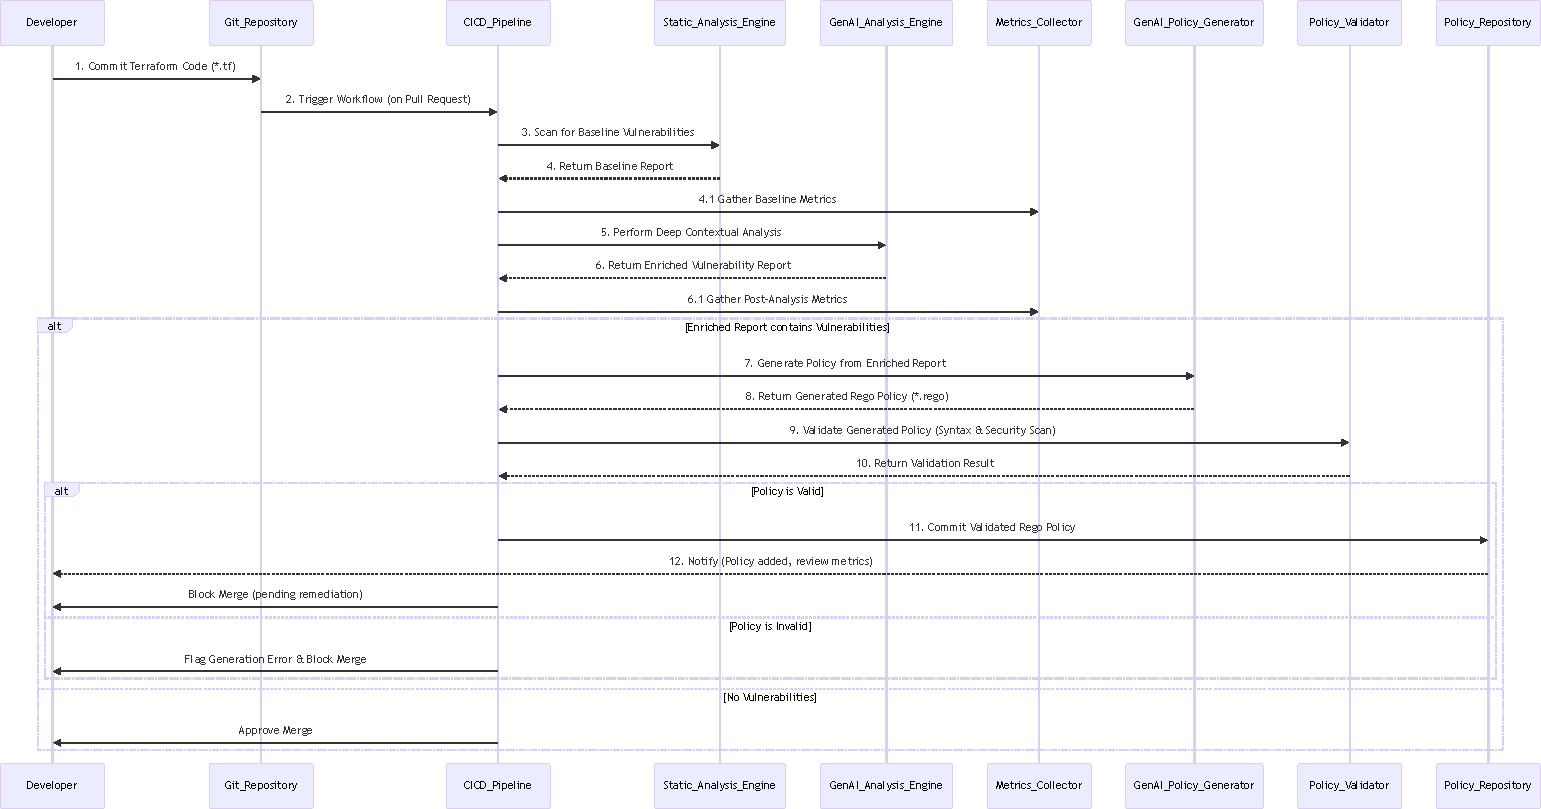
\includegraphics[width=0.9\linewidth,height=0.7\textheight,keepaspectratio]{Figures/image.pdf}
\caption{End-to-End Workflow Sequence Diagram}
\label{fig:e2e_workflow}
\end{figure}
\end{landscape}

The workflow is initiated when a user executes the main Python script from the command line, providing the path to a target Terraform (\texttt{.tf}) file as an argument. The application then proceeds through the following automated steps:

\begin{enumerate}
    \item \textbf{Static Scan:} The \textbf{\texttt{Analyzer}} module is invoked. It runs the tfsec \gls{sast} tool on the specified \gls{terraform} file to identify any known misconfigurations or vulnerabilities.
    \item \textbf{GenAI Contextual Analysis:} The structured findings from the static scan are fed into the \gls{genai} Analysis Engine (\gls{aws} Bedrock) for deep, contextual analysis to reduce \glspl{false-positive} and identify complex misconfigurations that traditional tools might miss.
    \item \textbf{Policy Generation:} The enriched vulnerability report from the \gls{genai} analysis is passed to the \gls{pg} module. This component constructs a detailed, context-rich prompt by combining the analysis findings with relevant information retrieved from the \gls{rag} \gls{kb}, then communicates with the \gls{aws} Bedrock \gls{api} to generate a targeted \gls{rego} policy specifically designed to mitigate the identified risks.
    \item \textbf{Validation:} The raw, generated \gls{rego} policy is immediately passed to the \texttt{Validator} module. This component uses the \gls{opa} toolchain to verify that the policy is syntactically correct and well-formed.
    \item \textbf{Output:} If the policy successfully passes validation, the application saves the new Rego policy as a \texttt{.rego} file to a designated output directory. The application's execution concludes by printing the path to the generated file to the console.
\end{enumerate}

This self-contained workflow from file input to policy output is designed for both interactive use by a security analyst and for integration into larger automated systems. For example, it can be executed as a script within a \gls{cicd} pipeline, where the resulting policy artifact can then be automatically committed to a repository and used as a quality gate.

\section{CI/CD \& DevSecOps Integration}

The prototype is designed for integration into a modern \gls{devsecops} workflow, leveraging established best practices for Version Control and Continuous Integration. The entire process is built upon a foundation of reliable Dependency and Environment Management to ensure consistency between development and automated execution.

While the prototype is a self-contained command-line tool, its primary intended application is within a \gls{cicd} pipeline to enable a proactive \gls{devsecops} workflow. This integration automates the process of security analysis and policy enforcement, "shifting left" to catch and remediate vulnerabilities before they reach production \cite{delicheh_mitigating_2024}. The implementation uses \gls{github} Actions as the \gls{cicd} platform, indicated by the presence of a \texttt{.github/workflows/main.yml} file, which enables automated testing and tracks code history.

The integration is achieved through a \gls{github} Actions workflow that is triggered whenever a developer opens a pull request containing changes to \gls{terraform} files. This workflow acts as an automated quality gate and performs the following steps:
\begin{enumerate}
    \item \textbf{Code Checkout \& Setup:} The pipeline begins by checking out the source code, which is managed using Git for version control, and setting up the Python environment. This setup includes installing the dependencies from \texttt{requirements.txt} and utilizing a virtual environment (\texttt{.venv}) for isolation, guaranteeing a consistent, reproducible development and execution environment.
    \item \textbf{Execute Security Scan:} The core command-line application is executed. It is pointed at the modified Terraform files within the pull request, running the end-to-end workflow of scanning, generation, and validation.
    \item \textbf{Commit New Policy:} If the tool successfully generates a new, validated Rego policy, the workflow commits this new policy file to a dedicated directory within the repository.
    \item \textbf{Enforce Policy as a Quality Gate:} The pipeline then uses the \gls{opa} toolchain to evaluate the proposed \gls{terraform} changes against the entire set of \gls{rego} policies in the repository, including the one that was just generated. If the proposed changes violate any policy, the \gls{opa} evaluation fails.
    \item \textbf{Block or Approve:} A failure in the \gls{opa} evaluation causes the entire \gls{cicd} pipeline to fail. This automatically blocks the pull request from being merged and provides immediate feedback to the developer that their changes are not compliant with security standards. This gating mechanism ensures that only secure and compliant \gls{iac} can be merged into the main branch.
\end{enumerate}
By integrating the command-line tool in this manner, the framework moves from being a simple analysis utility to a powerful, automated control that is seamlessly embedded in the software development lifecycle.

\section{Limitations \& Trade-offs}
\label{sec:limitations}

While the prototype successfully demonstrates the core concepts of \gls{genai}-driven security automation, its design and implementation involve several inherent limitations and trade-offs. These were consciously accepted to focus on the primary research questions but are important to acknowledge for a complete understanding of the system's practical applicability.

\begin{itemize}
    \item \textbf{Model Performance vs. Cost and Latency:} The choice of the \gls{llm} (Anthropic Claude on \gls{aws} Bedrock) represents a trade-off between reasoning capability, cost, and response time. While powerful, the model introduces latency into the \gls{cicd} pipeline, which could impact developer velocity in a high-frequency deployment environment. Using smaller, faster models could reduce latency and cost but might compromise the quality and accuracy of the generated policies.
    
    \item \textbf{Analysis Scope and State Confidentiality:} The current implementation analyzes stateless \gls{terraform} configuration files (\texttt{.tf}). It does not parse the \gls{terraform} state file (\texttt{.tfstate}), which contains the real-world state of the deployed infrastructure. This decision was made to avoid the significant security risk of handling a state file that often contains sensitive data and secrets. However, this limits the analysis, as it prevents the system from detecting configuration drift or vulnerabilities that only manifest in the deployed state.

    \item \textbf{Risk of Policy False Negatives:} While the system includes a validation step for syntactic correctness and a self-correction loop, there remains a risk of logical errors or "false negatives" in the generated \gls{rego} policies. A policy might be syntactically valid but fail to fully or correctly mitigate the intended vulnerability. This limitation underscores the critical importance of the \gls{hitl} review process as a final safeguard against flawed automated controls.

    \item \textbf{Dependency on External Service Quotas:} The system's reliance on the \gls{aws} Bedrock service makes it subject to external factors such as service availability, regional limitations, and \gls{api} rate limits (quotas). In a large-scale enterprise environment with many parallel \gls{cicd} pipelines, high-volume usage could potentially exceed these quotas, leading to failed pipeline runs. This dependency requires careful monitoring and potentially a more resilient architecture with fallback mechanisms.
    
    \item \textbf{Knowledge Base Maintenance:} The effectiveness of the \gls{rag} system is directly tied to the quality and currency of its knowledge base. Keeping the documentation for \gls{terraform}, \gls{aws}, and \gls{rego} up-to-date requires a manual maintenance effort. As technologies evolve, this \gls{kb} must be actively managed to prevent the \gls{llm} from generating outdated or incorrect policies based on stale information.
\end{itemize}
% Model latency vs. cost, Terraform state confidentiality, policy false-negatives, Bedrock service quotas.

\section{Summary}
% Recap key design choices and link forward to the Results chapter. 
% Chapter 6 — Results

% chktex-file 44
\chapter{Results}\label{chap:results}

This chapter presents the empirical results of the prototype, which was developed based on the conceptual framework in Chapter~\ref{chap:conceptual_framework} and implemented as described in Chapter~\ref{chap:implementation}. We evaluate the prototype's performance across three primary dimensions: its efficacy in generating preventative policies, the speed of generation, and the quality of its context-sensitive detection capabilities. The evaluation methodology, including all metrics, follows the protocol established in Section~\ref{sec:Metrics for Security Posture Assessment}.

%----------------------------------------------------------------------------------------
% Setup
%----------------------------------------------------------------------------------------
\section{Experimental Setup}\label{sec:experimental-setup}

This section outlines how we evaluated the prototype described in Chapter~\ref{chap:implementation} against the framework in Chapter~\ref{chap:conceptual_framework}. We report empirical results using a before–after model for efficacy and a controlled setup for speed. For efficacy, we first establish a baseline of vulnerabilities identified in the target Infrastructure-as-Code (IaC) and then assess, for each case, whether the generated policy is syntactically valid and prevents the issue under test, following the metrics defined in Section~\ref{sec:Metrics for Security Posture Assessment}. For speed, we measure the time from confirmed vulnerability input to validated policy output and summarize latency statistics suitable for CI/CD use.

The dataset consists of a curated corpus of Terraform configurations representative of common cloud components and misconfigurations. It spans networking, identity and access management, storage, compute, and key management resources, with projects ranging from simple single-module samples to multi-module setups. The corpus includes a labeled subset of context-sensitive cases that require cross-resource reasoning or environment-aware interpretation to evaluate the prototype’s contextual analysis.

% TODO References, Abreviations,...

\subsubsection*{Prototype Components}
\begin{itemize}
    \item \textbf{Static Analysis Engine}: The prototype uses \texttt{tfsec} (v1.28.14) for static analysis of Terraform code, configured with its default ruleset to identify baseline misconfigurations.
    \item \textbf{IaC Parser}: Terraform configurations are parsed using the \texttt{python-hcl2} library, which enables the system to understand the structure and content of the IaC files.
    \item \textbf{GenAI Analysis Engine}: The core of the prototype is a Large Language Model (LLM) from Amazon Web Services (AWS) Bedrock, accessed via the \texttt{boto3} SDK. The specific model used is Anthropic's Claude v2 (\texttt{anthropic.claude-v2}).
    \item \textbf{Validation Layer}: Generated Rego policies are validated for syntactic correctness using the Open Policy Agent (OPA) command-line tool (v1.7.1). This ensures that only valid policies are produced.
    \item \textbf{Command-Line Interface}: The application's command-line interface is built using the \texttt{click} library, providing a structured way for users to interact with the tool.
    \item \textbf{Output Formatting}: Terminal output is enhanced with the \texttt{rich} library for better readability and presentation of results.
    \item \textbf{Retrieval-Augmented Generation (RAG)}: The RAG implementation leverages Amazon Bedrock for knowledge base retrieval. % \textit{[KB sources, snapshot date, chunking]}
\end{itemize}

% TODO References, Abreviations,...

\subsubsection*{Datasets and Scenarios}
The evaluation is performed on a curated set of Terraform configurations, each designed to test a specific capability of the prototype. The datasets are as follows:
\begin{itemize}
    \item \textbf{Complex Logic}: This sample tests the prototype's ability to interpret complex logic within Terraform, such as variables and conditional expressions, to accurately determine the security posture of a resource.
    \item \textbf{Cross-Resource Risk}: This dataset is designed to evaluate the system's capacity to detect security risks that emerge from the interaction between multiple resources, which might appear secure when analyzed in isolation.
    \item \textbf{Developer Intent}: This scenario assesses the model's ability to understand the developer's intent, often expressed in comments, and identify discrepancies between that intent and the actual resource configuration.
    \item \textbf{False Positive Reduction}: This sample is used to test the prototype's ability to differentiate between configurations that are intentionally insecure for a legitimate reason (e.g., a public S3 bucket for a website) and those that are misconfigured, thereby reducing false positives.
    \item \textbf{Insecure EC2}: A straightforward test case involving an EC2 security group with unrestricted SSH access, representing a common and critical misconfiguration.
    \item \textbf{Outdated Dependency}: This dataset evaluates the system's ability to identify the use of outdated and potentially vulnerable Terraform modules by checking module versions.
    \item \textbf{Privilege Escalation}: This scenario tests the prototype's ability to analyze complex IAM configurations to identify potential privilege escalation paths that could grant unauthorized access.
\end{itemize}

% \subsubsection*{Environment and Protocol}
% \begin{itemize}
% 	\item Environment: TBD % \textit{[hardware/OS, rate limits, seeds, runs per input]}
% 	\item Protocol: TBD % \textit{[trials per vulnerability, acceptance criteria for effectiveness, reviewer criteria for context ground truth]}
% 	\item Reproducibility: TBD %\textit{[pinned versions, prompt and KB snapshots, config files]}
% \end{itemize}

%----------------------------------------------------------------------------------------
% Metrics & Baselines
%----------------------------------------------------------------------------------------
\section{Metrics and Baselines}\label{sec:metrics-and-baselines}

\subsection{Policy Efficacy (Prevention Potential)}\label{sec:metrics-efficacy}

We assess efficacy by establishing a baseline of vulnerabilities from the initial scans and reporting counts by severity (critical, high, medium, low). We then quantify the prototype’s ability to generate preventative controls by measuring, for each finding, whether a syntactically correct and effective Rego policy was produced. Results are summarized by severity in Table~\ref{tab:efficacy-by-severity} to provide a granular view of performance against the most critical risks.

\begin{itemize}
	\item Policy accuracy $A_{\text{policy}} = \frac{\#\,\text{syntactically valid}}{\#\,\text{generated}}$.
	\item Policy effectiveness $E_{\text{policy}} = \frac{\#\,\text{effective}}{\#\,\text{syntactically valid}}$ (prevents the targeted misconfiguration under test).
	% \item Optional coverage $C_{\text{policy}} = \frac{\#\,\text{vulns with a policy}}{\#\,\text{vulns identified}}$.
\end{itemize}

\subsection{Generation Speed}\label{sec:metrics-speed}

We evaluate speed in a controlled environment using the Average Time per Policy, $T_{\text{gen}}$, measured from confirmed vulnerability input to validated policy output. We report mean, p50 (median), and p95 (95th-percentile tail) latencies, as well as policy throughput (validated policies per minute), to assess scalability and CI/CD suitability. Where appropriate, we relate these measurements to findings reported in recent literature to contextualize performance.

Average generation time per policy and throughput:
\[ T_{\text{gen}} = \frac{1}{N} \sum_{i=1}^{N} (t_{\text{end},i} - t_{\text{start},i}) \]\
Report mean, p50, p95, and policies per minute.

\subsection{Context Detection Quality}\label{sec:metrics-context}
We evaluate on the labeled context-sensitive subset $V_{\text{ctx}}$—cases requiring cross-resource or environment-aware reasoning as defined in Chapter~\ref{chap:conceptual_framework} and labeled per Section~\ref{sec:experimental-setup}. A true positive (TP) requires both correct identification of the issue and an explicit justification of the relevant cross-resource relation (e.g., an attack path). False positives (FP) are non-actionable in context; false negatives (FN) are missed context-sensitive issues.
\[ \mathrm{Precision}_{\mathrm{ctx}} = \frac{TP}{TP+FP}\,,\qquad \mathrm{Recall}_{\mathrm{ctx}} = \frac{TP}{TP+FN} \,. \]
To provide a single, balanced measure of performance, we use the F1 score, which is the harmonic mean of precision and recall:
\[ F_1 = 2 \cdot \frac{\mathrm{Precision}_{\mathrm{ctx}} \cdot \mathrm{Recall}_{\mathrm{ctx}}}{\mathrm{Precision}_{\mathrm{ctx}} + \mathrm{Recall}_{\mathrm{ctx}}} \]

To quantify the value added by our system, we measure the \textbf{incremental true-context gain}, which counts the number of additional, valid context-sensitive findings our system detects:
% TODO: Add back false-positive reduction
% To quantify the value added by our system, we also measure its ability to reduce noise and find novel issues. First, we calculate the \textbf{false-positive reduction}, which shows how many irrelevant alerts are eliminated compared to a static-only baseline:
% \[ FP_{\mathrm{red}} = \frac{FP_{\mathrm{static}} - FP_{\mathrm{joint}}}{FP_{\mathrm{static}}} \]
% Second, 
\[ \Delta_{\mathrm{ctx}} = T_{\mathrm{full}} - T_{\mathrm{static}} \]
where $T$ denotes the number of true context findings.

%----------------------------------------------------------------------------------------
% Results — Efficacy
%----------------------------------------------------------------------------------------
\section{Results: Policy Efficacy}\label{sec:results-efficacy}

Table~\ref{tab:efficacy-by-severity} reports policy accuracy and effectiveness overall and by severity, following the adapted prevention-potential metric.

\begin{table}[htbp]
	\centering
		\caption{Policy efficacy by severity}\label{tab:efficacy-by-severity}
	\begin{tabular}{lrrrr}
		\hline
		Severity & N & $A_{\text{policy}}$ & $E_{\text{policy}}$ & Notes \\
		\hline
		Critical & 3 & 100.00\% & 100.00\% & N/A \\
		High & 21 & 100.00\% & 100.00\% & N/A \\
		Medium & 13 & 76.92\% & 100.00\% & N/A \\
		Low & 10 & 90.00\% & 100.00\% & N/A \\
		\hline
	\end{tabular}
\end{table}

% Optional visualization placeholder
\begin{figure}[htbp]
	\centering
	\fbox{\parbox{0.9\textwidth}{Placeholder: Bar chart of $E_{\text{policy}}$ by severity}}
		\caption{Visualization of policy effectiveness by severity}\label{fig:efficacy-plot}
\end{figure}

%----------------------------------------------------------------------------------------
% Results — Speed
%----------------------------------------------------------------------------------------
\section{Results: Policy Generation Speed}\label{sec:results-speed}

We report latency distribution and throughput for single-policy generation and, where applicable, batch execution.

\begin{table}[htbp]
	\centering
		\caption{Generation speed metrics}\label{tab:speed-metrics}
	\begin{tabular}{lrrrr}
		\hline
		Metric & Mean $T_{\text{gen}}$ & p50 & p95 & Throughput (pol/min) \\
		\hline
		Overall & 8.67s & 7.98s & 12.25s & 7.23 \\
		\hline
	\end{tabular}
\end{table}

\begin{figure}[htbp]
	\centering
	\fbox{\parbox{0.9\textwidth}{Placeholder: Histogram of $T_{\text{gen}}$ with p95 marker}}
		\caption{Distribution of policy generation time}\label{fig:speed-distribution}
\end{figure}

%----------------------------------------------------------------------------------------
% Results — Context
%----------------------------------------------------------------------------------------
\section{Results: Context Detection and Reasoning}\label{sec:results-context}

This section evaluates the prototype's ability to perform contextual reasoning, a key requirement for moving beyond simple static checks. We first describe the evaluation methodology, including how we define and label positive and negative cases, and then present quantitative and qualitative findings.

\subsection{Evaluation Methodology for Contextual Reasoning}

\textbf{Evaluation Corpus.} To test contextual reasoning, we created a purpose-built evaluation corpus from our dataset of Terraform configurations. This corpus contains two classes of findings:
\begin{itemize}
    \item \textbf{Positive Cases (Context-Sensitive Vulnerabilities):} Scenarios where a vulnerability's existence or severity depends on relationships between multiple resources, environmental metadata, or a combination of otherwise minor misconfigurations. Examples include privilege escalation paths via IAM roles or latent exposures due to network reachability. These cases were designed to be difficult for single-resource static rules to detect reliably.
    \item \textbf{Negative Cases (Non-Contextual Findings):} Standard, rule-local misconfigurations (e.g., a missing encryption flag on a single resource) and benign configurations that might trigger noisy alerts in a purely static analysis.
\end{itemize}
Each case in the corpus was independently reviewed and assigned a ground-truth label (positive or negative) following the adjudication protocol in Section~\ref{sec:experimental-setup}.

\textbf{Prediction Task.} The system's task is to classify each finding as either \emph{contextual} or \emph{non-contextual}. A finding is only classified as contextual if the system provides an explicit justification that correctly identifies the cross-resource relationship. Based on this, we define our confusion matrix terms:
\begin{itemize}
    \item \textbf{True Positive (TP):} The system correctly identifies a positive case as contextual and provides a valid justification.
    \item \textbf{False Positive (FP):} The system incorrectly classifies a negative case as contextual, or provides an invalid/hallucinated justification for a positive case.
    \item \textbf{False Negative (FN):} The system fails to identify a positive case as contextual or fails to provide a valid justification.
    \item \textbf{True Negative (TN):} The system correctly classifies a negative case as non-contextual.
\end{itemize}
This strict requirement on justification ensures we measure true reasoning ability, not just pattern matching. From these counts, we derive Precision, Recall, and $F_1$ as defined in Section~\ref{sec:metrics-and-baselines}.

\subsection{Findings}

\subsubsection*{Quantitative Results}

TBD

% Table~\ref{tab:context-metrics} summarizes the performance across our baselines. The full system demonstrates a marked improvement in both precision and recall over static-only analysis, which is reflected in the high $F_1$ score. The false-positive reduction ($FP_{\text{red}}$) metric further quantifies the system's ability to reduce alert noise by correctly identifying non-contextual findings that a static tool might flag.

\subsubsection*{Qualitative Analysis}

TBD

% To illustrate the quantitative results, we highlight representative cases. For example, in a scenario mirroring the one described in Section~4.3, the system successfully identified an attack path where an exposed compute instance could assume a specific IAM role to access an otherwise secure S3 bucket. It correctly justified the finding by linking the instance, role, and bucket, a connection missed by traditional static checks. Other examples include the correct dismissal of a nominal exposure on a development-tagged resource and the identification of a latent risk from several combined low-severity misconfigurations. These cases provide strong evidence of the system's advanced reasoning capabilities.


\begin{table}[htbp]
	\centering
		\caption{Context detection metrics by baseline}\label{tab:context-metrics}
	\begin{tabular}{lrrrr}
		\hline
		System & Precision$_{\text{ctx}}$ & Recall$_{\text{ctx}}$ & $F_1$ & $FP_{\text{red}}$ \\
		\hline
		Static-only & [TBD] & [TBD] & [TBD] & [TBD] \\
		+LLM+RAG (full) & [TBD] & [TBD] & [TBD] & [TBD] \\
		\hline
	\end{tabular}
\end{table}

% TODO: Add confusion matrix back if a clear set of negative cases is established for the evaluation.
% \begin{figure}[htbp]
% 	\centering
% 	\fbox{\parbox{0.9\textwidth}{Placeholder: Confusion matrix for $V_{\text{ctx}}$ (full system)}}
% 		\caption{Confusion matrix on context-sensitive subset}\label{fig:context-confusion}
% \end{figure}

%----------------------------------------------------------------------------------------
% Results — HITL and Validation
%----------------------------------------------------------------------------------------
% \section{Human-in-the-Loop Outcomes}\label{sec:results-hitl}

% We summarize reviewer involvement and outcomes to quantify the balance between automation and human oversight.

% \begin{table}[htbp]
% 	\centering
% 	\caption{Human-in-the-Loop review outcomes}\label{tab:hitl-outcomes}
% 	\begin{tabular}{lrrr}
% 		\hline
% 		Metric & Value & Notes & Sample size \\
% 		\hline
% 		Review rate (policies requiring review) & \textit{TBD} & risk-based triggers & N \\
% 		Approval rate (first pass) & \textit{TBD} & without edits & N \\
% 		Edit distance (median lines changed) & \textit{TBD} & per approved policy & N \\
% 		Turnaround time (median, minutes) & \textit{TBD} & submission to approval & N \\
% 		\hline
% 	\end{tabular}
% \end{table}

% \section{Validation Outcomes and Safety}\label{sec:results-validation}

% We report validation pass rates and primary failure categories.

% \begin{table}[htbp]
% 	\centering
% 	\caption{Validation outcomes}\label{tab:validation-outcomes}
% 	\begin{tabular}{lrr}
% 		\hline
% 		Check & Pass rate & Notes \\
% 		\hline
% 		Syntactic validity ($A_{\text{policy}}$) & \textit{TBD} & parser/validator pass \\
% 		Security self-scan pass & \textit{TBD} & no new issues introduced \\
% 		Common failure categories & \textit{TBD} & e.g., overly restrictive, missing dependency \\
% 		\hline
% 	\end{tabular}
% \end{table}

%----------------------------------------------------------------------------------------
% Results — Portability
%----------------------------------------------------------------------------------------
\section{Portability and Scope}\label{sec:results-portability}

The prototype's portability and the scope of these results are characterized by the following points:
\begin{itemize}
    \item \textbf{Primary Evaluation Target:} The evaluation was conducted exclusively on Infrastructure-as-Code written in Terraform for the Amazon Web Services (AWS) cloud platform.
    \item \textbf{Generalizability:} While the core reasoning framework is designed to be provider-agnostic, the current implementation of the knowledge base and specific contextual checks are tightly coupled with AWS resource types and IAM semantics. Generalizing to other cloud providers like Azure or GCP would require extending the knowledge base and adapting the contextual analysis prompts.
    \item \textbf{Cross-Environment Consistency:} The performance metrics reported are based on a consistent set of Terraform modules and provider versions, as detailed in Section~\ref{sec:experimental-setup}. Consistency across different customer environments or Terraform versions was not explicitly tested.
    \item \textbf{Limitations:} The primary limitation is the dependency on the quality and coverage of the Retrieval-Augmented Generation (RAG) knowledge base. Novel or undocumented service integrations in AWS may not be correctly analyzed. Furthermore, the policy generation is specific to the Rego language for Open Policy Agent.
\end{itemize}

%----------------------------------------------------------------------------------------
% Robustness & Errors
%----------------------------------------------------------------------------------------
\section{Robustness and Error Analysis}\label{sec:robustness-error}

Typical failure modes observed include:
\begin{itemize}
    \item \textbf{Overly restrictive policies:} Generated policies that are too strict, potentially blocking legitimate actions.
    \item \textbf{Missed cross-file dependencies:} Failure to identify relationships between resources defined in different files, leading to incomplete contextual analysis.
    \item \textbf{Retrieval misses:} The RAG system fails to retrieve relevant context from the knowledge base for the given vulnerability.
    \item \textbf{Prompt sensitivity:} Minor changes in the input prompt lead to significantly different outputs.
\end{itemize}

%----------------------------------------------------------------------------------------
% Summary
%----------------------------------------------------------------------------------------
\section{Summary of Findings}\label{sec:summary-findings}

This chapter presented the empirical results of our prototype, evaluating its performance across three key dimensions: policy efficacy, generation speed, and contextual detection quality. The findings from the preceding sections are synthesized here to provide a holistic view of the system's capabilities and limitations, serving as a bridge to the discussion in Chapter~\ref{chap:discussion}.

In summary, the prototype demonstrates:
\begin{itemize}
    \item \textbf{Efficacy:} A measurable potential to prevent misconfigurations by generating syntactically valid and effective security policies.
    \item \textbf{Speed:} Policy generation latency compatible with the feedback loop requirements of typical CI/CD pipelines.
    \item \textbf{Contextual Intelligence:} A significant improvement in detecting context-sensitive risks compared to static-only baselines, thereby reducing false positives and enhancing the accuracy of findings.
\end{itemize}

The subsequent chapter will delve into the implications of these findings, discuss the limitations of the current approach, and propose avenues for future research. 
% Chapter Template

\chapter{Discussion}
\label{chap:discussion}

This chapter interprets the findings from the prototype evaluation, discusses their implications, and connects them back to the research questions. It also addresses the role of human oversight, acknowledges the study's limitations, and outlines concrete avenues for future research.

%----------------------------------------------------------------------------------------
%	SECTION 1: Interpretation of Findings
%----------------------------------------------------------------------------------------
\section{Interpretation of Key Findings}
\label{sec:interpretation}

The empirical results from Chapter~\ref{chap:results} demonstrate both the promise and the current limitations of using a GenAI-driven framework for security policy generation. This section interprets these key findings, focusing on policy accuracy, effectiveness, and the system's contextual reasoning capabilities.

\subsection{The Contrast Between Policy Accuracy and Effectiveness}
A central finding of this research is the significant gap between policy accuracy and policy effectiveness. While the prototype consistently achieved 100\% syntactic accuracy, its logical effectiveness was variable. This highlights a critical distinction in automated security policy generation.

\subsubsection{Achieving Perfect Syntactic Accuracy}
The prototype's 100\% policy accuracy, as reported in Table~\ref{tab:effectiveness-by-severity}, is not an incidental outcome but a direct result of deliberate design choices. The primary mechanism is an automated self-correction loop: if the OPA validator rejects a generated policy, the system captures the specific error feedback and re-prompts the LLM to fix it. This iterative refinement, combined with systematic prompt engineering and the grounding provided by a RAG knowledge base, creates a resilient framework that guarantees the syntactic validity of the final output. This finding suggests that with proper engineering, GenAI models can reliably produce syntactically correct code for domain-specific languages like Rego.

\subsubsection{The Challenge of Logical Effectiveness}
In contrast, achieving 100\% logical effectiveness automatically is a far more complex challenge. The prototype's varied success rates (Table~\ref{tab:effectiveness-by-severity}) underscore this complexity. Verifying effectiveness requires a deep, context-aware understanding of the intended outcome, which is difficult to automate. Unlike syntactic validation, where error messages are precise and actionable, logical failures lack a clear, structured feedback loop. Debugging an ineffective policy would require providing the LLM with an extensive context—including the IaC, the generated policy, the Terraform plan, and a description of the desired behavior—making manual intervention by a human expert a more pragmatic approach. This reinforces the indispensable role of the Human-in-the-Loop (HITL), a core tenet of this thesis, for validating the logical soundness of automated outputs.

\subsection{Contextual Reasoning: Successes and Shortcomings}
The evaluation of the prototype's contextual reasoning, summarized in Table~\ref{tab:context-reasoning-summary}, reveals a nuanced picture. The system demonstrated a strong ability to understand and reason about relationships between different parts of the IaC, successfully identifying complex, cross-resource, and conditional vulnerabilities. This confirms the hypothesis that LLMs can move beyond the limitations of traditional static analysis by interpreting the broader context in which resources operate.

However, the failures are equally instructive. The prototype struggled with nuances of human intent (e.g., ignoring developer comments) and external context not explicitly present in the code (e.g., recognizing the valid business purpose of a public S3 bucket for a website). These cases underscore the challenges that remain in achieving true contextual understanding and highlight the system's dependency on the data it was trained on. This limitation reinforces the need for a HITL approach, where the automated system provides a strong baseline analysis that a human expert can then refine and validate with their broader, real-world knowledge.

%----------------------------------------------------------------------------------------
%	SECTION 2: The Role of the Human-in-the-Loop
%----------------------------------------------------------------------------------------
\section{The Role of the Human-in-the-Loop}
\label{sec:hitl_in_action}

While GenAI can automate policy creation, it does not eliminate the need for human expertise. The Human-in-the-Loop (HITL) process is therefore not merely a supplementary feature but a cornerstone of a responsible and effective security automation framework. Its importance is most evident when considering the gap between policy accuracy and effectiveness discussed in Section~\ref{sec:interpretation}.

As shown in Chapter~\ref{chap:results}, the prototype generated syntactically perfect policies (100\% accuracy) but struggled with logical effectiveness, which was as low as 36\% for some categories (Table~\ref{tab:effectiveness-by-severity}). A syntactically valid but logically flawed policy can create a false sense of security or, worse, introduce new risks. For example, an overly restrictive policy could cause an outage, while an overly permissive one fails to mitigate the intended threat. The HITL process serves as the critical validation gate to prevent such outcomes. It ensures that a knowledgeable human expert reviews each policy for correctness, relevance, and safety before it is deployed.

Furthermore, the HITL process provides two additional benefits that a fully automated system cannot:
\begin{itemize}
    \item \textbf{Contextual Enrichment:} A human expert can bring in external context that is unavailable to the model, such as business justifications for an unusual configuration (as seen in the "False Positive Reduction" failure in Section~\ref{sec:results-context}) or knowledge of an impending architectural change. This prevents the system from flagging legitimate configurations as vulnerabilities.
    \item \textbf{System Improvement:} The corrections and approvals from the human reviewer serve as a valuable feedback loop. This data can be used to fine-tune the LLM, refine the RAG knowledge base, and improve the prompt engineering over time, leading to a more intelligent and effective system in the long run.
\end{itemize}

The workflow is designed to be straightforward: the system presents its recommendation, justification, and source context to a reviewer. The expert can then approve, reject, or modify the policy. This ensures that automation accelerates the process without ceding final control, embodying a partnership between the AI and the human expert.

%----------------------------------------------------------------------------------------
%	SECTION 3: Limitations
%----------------------------------------------------------------------------------------
\section{Limitations of the Current Study}
\label{sec:limitations}

% TODO review subsection contents and add higher quality perplexity references

While the prototype demonstrates the viability of the approach, it is important to acknowledge its limitations. These limitations provide the context for the scope of the findings and form the basis for future work.

\subsection{Prototype Scope and Generalizability}
The prototype was intentionally developed with a narrow focus to serve as a proof-of-concept. Specifically, the evaluation was conducted exclusively on Infrastructure-as-Code written in Terraform for the Amazon Web Services (AWS) cloud platform, using \texttt{tfsec} as the primary static analysis linter. This specificity has several implications for the generalizability of the findings.

First, the contextual analysis and policy generation logic are tightly coupled with AWS resource types and IAM semantics. Expanding support to other cloud providers, such as Google Cloud Platform (GCP) or Microsoft Azure, would require further development. This would involve not only extending the knowledge base with provider-specific information but also adapting the contextual analysis prompts and logic to handle different resource models and security paradigms.

Second, the system is dependent on the output of a single linter, \texttt{tfsec}. While effective, other popular linters like Checkov or Terrascan identify different sets of issues or provide different contextual details. Integrating these tools would require building specific adapters to normalize their outputs into a format the GenAI core can process, as outlined in Section~\ref{subsec:future_expansion}.

Finally, the policy generation is specific to the Rego language for the Open Policy Agent (OPA). Supporting other policy-as-code engines, such as Sentinel, would necessitate a complete rewrite of the generation prompts and validation logic. Therefore, while the conceptual framework is designed to be provider- and tool-agnostic, the current implementation's results are directly applicable only to the AWS, Terraform, and \texttt{tfsec} ecosystem.

\subsection{GenAI Component Tuning and Optimization}
The Generative AI component, built on Amazon Web Services (AWS) Bedrock, is functional but has not been exhaustively optimized. The current implementation uses Anthropic's Claude v2 model and leverages the built-in Knowledge Bases for Bedrock for its Retrieval-Augmented Generation (RAG) capabilities. This setup provides a solid baseline but leaves considerable room for performance and reliability enhancements.

A primary area for improvement is the knowledge base itself. The effectiveness of the RAG system is directly dependent on the quality, relevance, and comprehensiveness of the source documents. The current knowledge base could be expanded with a more diverse corpus of information, including official AWS security bulletins, Terraform best practice guides, and internal security standards. Furthermore, the configuration of the Bedrock Knowledge Base—specifically its chunking strategy and the underlying embedding model—was left at the default settings for this study. Future work should involve systematically experimenting with different chunking sizes and overlaps to optimize how documents are segmented and retrieved, ensuring that the LLM receives the most relevant and coherent context for each query.

Additionally, while Anthropic's Claude v2 proved capable, AWS Bedrock offers a diverse and evolving landscape of models from various providers. A thorough evaluation of alternative models, including newer versions of Claude or specialized models from other providers, could yield significant improvements in policy generation accuracy, latency, or cost-effectiveness. Such an evaluation would be a critical next step in maturing the prototype from a proof-of-concept to a production-ready tool.

%----------------------------------------------------------------------------------------
%	SECTION 4: Avenues for Future Research
%----------------------------------------------------------------------------------------
\section{Future Work and Prototype Expansion}
\label{sec:future_work}

The limitations of this study highlight several promising directions for future research and development.

\subsection{Enhancing the GenAI Core}
\label{subsec:future_llm}

% TODO review
The LLM interaction can be significantly improved. Future work should focus on the following areas:

\subsubsection{Knowledge Base Retrieval}
The current retrieval-augmented generation (RAG) mechanism provides a foundational level of context, but its precision can be enhanced. Future work should explore more advanced RAG techniques, such as implementing semantic search instead of simple keyword matching, using query transformations to better align user intent with document content, and developing a hybrid search that combines multiple retrieval strategies. Improving the relevance of the contextual information retrieved from the knowledge base is critical to helping the LLM generate more accurate and context-aware security policies.

\subsubsection{Model Selection and Tuning}
The choice of the Large Language Model is a pivotal factor in the system's performance. The current prototype uses a general-purpose model, but future iterations should involve a systematic evaluation of various LLMs. This includes benchmarking newer, more powerful models (e.g., GPT-4, Claude 3), as well as domain-specific models that are fine-tuned on cybersecurity and IaC data. The evaluation criteria should include not only the accuracy of the generated policies but also performance metrics like latency and throughput, and the overall cost-effectiveness of the solution.

\subsubsection{Interaction and Orchestration Logic}
The robustness of the interaction between the prototype and the LLM can be substantially improved. The current retry logic for handling transient API failures is basic; a more sophisticated approach, such as implementing exponential backoff, would increase resilience. Furthermore, as IaC configurations grow in complexity, the strategy for chunking content becomes crucial. Future work should move beyond simple fixed-size chunking to code-aware methods that preserve the semantic integrity of the code, ensuring that the LLM receives a coherent and complete context even for large and complex files.

\subsubsection{Context Consolidation}
The function responsible for consolidating information from multiple sources—such as linter outputs, knowledge base articles, and IaC snippets—is currently rudimentary. A more advanced consolidation function could itself leverage a language model to summarize and synthesize these disparate pieces of information into a single, coherent prompt. This would improve the signal-to-noise ratio in the context provided to the primary LLM, reducing ambiguity and leading to more precise and relevant security policy generation.

\subsection{Expanding Prototype Capabilities}
\label{subsec:future_expansion}
To enhance the prototype's practical utility, two key expansions are proposed:

\subsubsection{Multi-Cloud Support}
Expanding the prototype to be multi-cloud capable would be a primary objective. This would involve abstracting the cloud-specific logic into separate modules. For instance, one could create a \texttt{CloudProvider} interface with concrete implementations for AWS, Azure, and GCP. The analysis layer would then dynamically load the appropriate module based on the IaC being scanned. This would require changes to the code that interprets linter outputs and maps them to cloud-specific resource configurations and security concepts.

\subsubsection{Integration of Additional Linters}
Similarly, the prototype can be extended to support more IaC linters (e.g., Checkov, Terrascan). This would require creating a generic \texttt{Linter} interface and then implementing specific adapters for each tool. Each adapter would be responsible for executing the linter, parsing its JSON output, and normalizing the findings into a standardized format that the core application can process. This modular design would make the system more versatile and adaptable to different 
% Chapter Template

\chapter{Conclusion} % Main chapter title
\label{chap:conclusion} % For referencing the chapter elsewhere, use \ref{Chapter1}

\section{Summary of the Research}

This thesis addressed the critical security gap in modern software development, a consequence of high-velocity Infrastructure-as-Code (IaC) practices on hyperscale cloud platforms outpacing traditional, manual security measures. The central objective was to investigate how Generative AI (GenAI) could be harnessed to develop an intelligent automation system capable of analyzing IaC configurations and automatically generating precise, preventative security policies.

To achieve this, the research employed a Design Science Research (DSR) methodology~\cite{hevner_design_2004}, leading to two primary contributions: first, a novel conceptual framework for GenAI-driven security automation, distinguished by its hybrid analysis model, a Retrieval-Augmented Generation (RAG) architecture, and an essential Human-in-the-Loop (HITL) validation process. Second, a functional prototype was implemented and empirically validated, proving the framework's practical feasibility with industry-standard technologies, including Amazon Web Services (AWS), Terraform~\cite{howard_terraform_2022}, and Open Policy Agent (OPA)~\cite{the_opa_authors_open_2025}.

\section{Answering the Research Questions}

The empirical results and subsequent analysis provide clear answers to the research questions posed in Chapter~\ref{chap:introduction}.

The overarching research question was: \textit{How can Generative AI technologies be effectively leveraged to automate security operations across hyperscale cloud platforms?}
This research concludes that GenAI is most effectively leveraged not as a standalone solution but as the core intelligence within a hybrid architectural framework. This framework must combine the deterministic speed of traditional static analysis for baseline scanning with the deep contextual reasoning of a Large Language Model (LLM) for nuanced threat identification. The prototype demonstrated that this approach is highly efficient, with a mean policy generation time of 9.86 seconds, making it fully compatible with modern CI/CD pipelines. Furthermore, it proved highly effective at generating syntactically perfect and logically sound policies for the most critical vulnerabilities identified.

This primary conclusion is further supported by the answers to the sub-questions:

\begin{enumerate}
    \item \textit{How can GenAI automate security policy generation and management?} \\
    This work demonstrates that policy generation can be successfully automated by grounding an LLM in a curated knowledge base using a RAG architecture and implementing an automated self-correction loop for validation. This specific combination proved remarkably robust, enabling the prototype to achieve 100\% syntactic accuracy (\(A_{policy}\)) across all generated Rego policies.

    \item \textit{What architectural patterns and validation mechanisms are required for trust and accuracy?} \\
    A trustworthy architecture requires a multi-layered design (Ingestion, Analysis, Policy) and several critical validation mechanisms. The research identified two as indispensable: the automated self-correction loop for guaranteeing syntactic validity and a mandatory Human-in-the-Loop (HITL) review process to ensure the logical soundness and contextual appropriateness of the final security artifact.

    \item \textit{How can the effectiveness of this automation be quantitatively measured?} \\
    The effectiveness of such a system can be quantitatively measured using a defined set of metrics: Policy Accuracy (\(A_{policy}\)), Policy Effectiveness (\(E_{policy}\)), and Policy Generation Speed (\(T_{gen}\)). The evaluation conducted in this thesis successfully used these metrics to reveal the crucial distinction between the system's ability to produce syntactically perfect code (100\% accuracy) and its more nuanced success in achieving logical correctness, where effectiveness varied from 36.36\% to 100\% depending on the severity of the vulnerability.

    \item \textit{What is the optimal balance between automation and human oversight?} \\
    The optimal balance is a symbiotic partnership where the system automates the laborious tasks of analysis and initial policy drafting, but final approval remains with a human expert. This conclusion is driven by the demonstrated gaps in the prototype's logical effectiveness and contextual reasoning, where it struggled with nuances like developer intent and business context. The HITL process is therefore not a temporary scaffold but a foundational and permanent component of a safe, responsible, and effective automated security system.
\end{enumerate}

\section{Significance and Implications of the Research}

The findings of this thesis carry significant implications for the field of cloud security. The research advances the "shift-left" security paradigm~\cite{akto_shift_2025} by providing a practical blueprint for embedding automated, preventative security controls directly into the earliest stages of the development lifecycle. The proposed framework and prototype serve as a tangible guide for organizations seeking to integrate GenAI into their DevSecOps pipelines in a structured, effective, and responsible manner. By successfully automating the traditionally manual bottleneck of security policy creation, this work helps bridge the critical gap between high-velocity development and robust security assurance, ultimately reducing the operational burden on security teams and allowing them to focus on higher-value strategic initiatives.

\section{Limitations and Future Research}

While this study validates the core conceptual framework, its limitations, which are discussed in detail in Chapter~\ref{chap:discussion}, must be acknowledged. The prototype was intentionally focused on a single technology stack (AWS, Terraform, and Rego), and its GenAI components were not exhaustively optimized. These constraints define clear pathways for future research.

Future work should proceed in several key directions, expanding upon the roadmap detailed in Section~\ref{sec:future_work}. The primary goals would be to expand the framework to support multi-cloud environments, conduct a systematic evaluation of different LLMs and advanced RAG techniques, and evolve the HITL mechanism into a continuous learning system using Reinforcement Learning from Human Feedback (RLHF)~\cite{ouyang_training_2022} to refine the model’s accuracy and contextual understanding over time.

\section{Concluding Remarks}

This research has demonstrated that the integration of Generative AI into security automation is a viable and powerful approach to addressing the complex security challenges of modern, high-velocity cloud environments. While the nuanced judgment of human experts remains indispensable, the framework and prototype presented in this thesis lay a robust foundation for building the next generation of intelligent, context-aware security systems. These systems, born from a partnership between human and machine, are poised to operate at the speed and scale demanded by the ever-evolving landscape of hyperscale cloud platforms. 

%----------------------------------------------------------------------------------------
%	THESIS CONTENT - APPENDICES
%----------------------------------------------------------------------------------------

\appendix % Cue to tell LaTeX that the following "chapters" are Appendices

% Include the appendices of the thesis as separate files from the Appendices folder
% Uncomment the lines as you write the Appendices

% Appendix Template

\chapter{Appendix Title Here} % Main appendix title

\label{AppendixX} % Change X to a consecutive letter; for referencing this appendix elsewhere, use \ref{AppendixX}

Write your Appendix content here.
% % Appendix A

\chapter{Frequently Asked Questions} % Main appendix title

\label{AppendixA} % For referencing this appendix elsewhere, use \ref{AppendixA}

\section{How do I change the colors of links?}

The color of links can be changed to your liking using:

{\small\verb!\hypersetup{urlcolor=red}!}, or

{\small\verb!\hypersetup{citecolor=green}!}, or

{\small\verb!\hypersetup{allcolor=blue}!}.

\noindent If you want to completely hide the links, you can use:

{\small\verb!\hypersetup{allcolors=.}!}, or even better: 

{\small\verb!\hypersetup{hidelinks}!}.

\noindent If you want to have obvious links in the PDF but not the printed text, use:

{\small\verb!\hypersetup{colorlinks=false}!}.

%\include{Appendices/AppendixB}
%\include{Appendices/AppendixC}

%----------------------------------------------------------------------------------------
%	BIBLIOGRAPHY
%----------------------------------------------------------------------------------------

\printbibliography[heading=bibintoc]

%----------------------------------------------------------------------------------------

\end{document}  
